\documentclass{article}
\usepackage[utf8]{inputenc}
\usepackage{amsmath,amsthm,amssymb,graphicx,setspace,mathrsfs,mathstyle,listings,color}
\usepackage{csvsimple}
%\topmargin 0in
%\headheight 0in
%\headsep .2in
%\textheight 220mm
%\textwidth 159mm
%\oddsidemargin 0in
%\evensidemargin 0in

\newtheorem{theorem}{Theorem}[section]
\newtheorem{lemma}[theorem]{Lemma}
\newtheorem{proposition}[theorem]{Proposition}
\newtheorem{conjecture}[theorem]{Conjecture}
\newtheorem{question}[theorem]{Question}
\newtheorem{corollary}{Corollary}[theorem]

\theoremstyle{definition}
\newtheorem{definition}{Definition}
\newtheorem{example}{Example}

\theoremstyle{remark}
\newtheorem{remark}{Remark}

\numberwithin{equation}{section}

\definecolor{codegreen}{rgb}{0,0.6,0}
\definecolor{codegray}{rgb}{0.5,0.5,0.5}
\definecolor{codepurple}{rgb}{0.58,0,0.82}
\definecolor{backcolour}{rgb}{0.95,0.95,0.92}
 
\lstdefinestyle{mystyle}{
    backgroundcolor=\color{backcolour},   
    commentstyle=\color{codegreen},
    keywordstyle=\color{magenta},
    numberstyle=\tiny\color{codegray},
    stringstyle=\color{codepurple},
    basicstyle=\footnotesize,
    breakatwhitespace=false,         
    breaklines=true,                 
    captionpos=b,                    
    keepspaces=true,                 
    numbers=left,                    
    numbersep=5pt,                  
    showspaces=false,                
    showstringspaces=false,
    showtabs=false,                  
    tabsize=2
}

\lstset{style=mystyle}

\title{The Ulam sequence and related phenomena}
\author{Daniel Ross}
\date{ }

\begin{document}
\maketitle

\tableofcontents

\section{Introduction}

The Ulam sequence is a sequence of positive integers that is defined
in a recursive way that sounds like it should make it difficult to
compute.  It starts with $a_1 = 1$, $a_2 = 2$, and then for $n > 2$,
$a_n$ is the integer satisfying: 
\begin{enumerate}
\item It is expressible as a sum of distinct previous terms in exactly
  one way: There is exactly one pair of $i < j$ with
  $a_i + a_j = a_n$.
\item It is larger than the previous element of the sequence: $a_n >
  a_{n-1}$.
\item It is the smallest positive integer with the above two
  properties.
\end{enumerate}

Thus the first few terms can be computed: 

\[1, 2, 3, 4, 6, 8, 11, 13, 16, 18, 26, 28, 36, 38, 47, 48, 53, 57, 62,
69, \ldots\]

In particular, there are two ways a number could fail to be Ulam:
Either it has a representation as a sum of two distinct smaller Ulam
numbers in more than one way (such as $5 = 4+1 = 2+3$), or it has no
representations as a sum of distinct smaller Ulam numbers at all (such
as 23).

One thing that makes the sequence interesting is that it seems
historically to have been very difficult to prove anything about it.
We know, for example, that it must be infinite, since, given the first
$n$ elements $a_1, \ldots, a_n$, we can always find at least one
number that satisfies both the criteria above, namely $a_{n-1} + a_n$.
Thus there must be a smallest such number, which is therefore the next
Ulam number.

We also know that if we use the same definition but start with
different initial values, we can get sequences that we can analyse
very easily indeed: If the $(u,v)$-Ulam sequence is the sequence with
$a_1 = u, a_2 = v$, and $a_n$ (for $n > 3$) defined exactly as before,
then by theorems of Finch \cite{regularity_criterion_finch} and Schmerl and Speigel \cite{regularity_schmerl}, we
know that the $(2,v)$-Ulam sequence, in the case where $v$ is odd and
at least 5, is regular in the following sense:

\begin{definition}\label{def:regularity}
  An increasing, infinite sequence $\{a_i\}$ of positive integers is
  \textbf{regular} if the sequence $\{b_i = a_i - a_{i-1} : i > 1\}$
  is eventually periodic.
\end{definition}

Such sequences are very easy to describe--we could specify them (after
some initial segment) by a set of congruence classes modulo some
(possibly large) $m$.  In particular, a regular Ulam-like sequence
will be far easier to compute than the definition of an Ulam sequence
would naively suggest.

There are other initial values that are variously known to and
believed to give rise to regular sequences, also.  See, for example,
\cite{patterns_finch}.  That said, many
Ulam-type sequences appear not to be regular, among them the $(1,2)$-
and $(2,3)$-Ulam sequences.  So one might ask some questions:

\begin{itemize}
\item What is it that causes some initial conditions to be regular and
  not others (if indeed they are not)?
\item Is there any perhaps more general notion of regularity that even
  the irregular-looking sequences do satisfy?
\end{itemize}

In looking for hidden regularity, one might take a signal processing
approach to the sequence and try, for example, to Fourier transform
the indicator function of the sequence and see if the spectrum has any
interesting features.  In \cite{ulam_steinerberger}, Stefan Steinerberger did exactly
that and behold, the spectrum has a large spike exactly only at some
$\alpha \in \R/\Z$ (and at its harmonics), and seemingly nowhere else.

More precisely: 

\begin{definition} If $f : [N] \to \C$, recall the the \textbf{Fourier
    transform} of $f$ is a function $\widehat{f}$ defined by the
  formula:

\[\widehat{f}(x) = \frac 1N \sum_{t=0}^{N-1} f(t) e(-tx)\]

where $e(x) = e_N(x) = e^{2\pi i x / N}$.  Thus $\widehat{f}$ is a
function defined on all of $\R/\Z$.

$N$ will often be omitted from the notation and understood from
context.  If we wish to make $N$ explicit in the notation for the
Fourier transform itself, we will denote it as $\mathcal{F}_N f$
rather than $\widehat{f}$.

\end{definition}

This definition satisfies many properties, which are standard from
Fourier analysis and additive combinatorics \cite{additive_combinatorics_tao}:

\begin{proposition}
If $f : [N] \to \C$, then: 

\begin{itemize}
\item If in fact $f$ takes values in $\R$, then
  $\widehat{f}(-x) = \overline{\widehat{f}(x)}$ for all $x \in \R/\Z$.

\item $\widehat{\widehat{f}}(x) = f(-x)$ for all $x \in [N]$.

\item $\widehat{fg}(x) = (\widehat{f} \ast \widehat{g})(x)$ for all
  $x \in \R/\Z$.

\item If in fact $f$ is the indicator function of a set
  $A \subseteq [N]$, then $\widehat{f}(0) = \frac{|A|}{N}$.
\end{itemize}
\end{proposition}

So if $A$ is a set of positive integers (say, the Ulam sequence), and
$1_A$ is the indicator function of $A$, then we might define
$\widehat{1_A}(x) = \lim_{N \to \infty} \widehat{1_{A_N}}(x)$, where
as usual, $A_N = A \cap [N]$ is the truncation of $A$ at $N$.  Then in
the case of the Ulam sequence, what is observed numerically is that
for one particular value of $\alpha \in \R/\Z$ (namely
$\alpha = \ldots)$, that $\widehat{1_A}(\alpha) \approx 0.8$, and for
$k \in \Z$, $\widehat{1_A}(k \alpha)$ is also some non-zero value that
shrinks with $k$.  For example, for $N = 100000$, we compute this for
a few values of $k$ (noting that of course the values for $-k$ are
just the conjugates of these:

\begin{tabular}{|l|l|}
\hline
  $k$ & $\widehat{A}(k\alpha)$
  \csvreader{datafiles/harmonics_u1_2.csv}{}
  {\\\csvcoli & \csvcolii}
\\\hline
\end{tabular}

and as $N$ gets large, it appears that
$\widehat{1_{A_N}}(\beta) \to 0$ as $N \to \infty$ for all other
$\beta \notin \alpha\Z$.

From a signal processing perspective, this might suggest that the set
$A$ has some periodicity mod $\frac 1 \alpha \approx \ldots$.  Using
$\ldots$ as a rational approximation to this, we can plot the
distribution of $A_N$ for, say, $N = 100000$ modulo this number: 

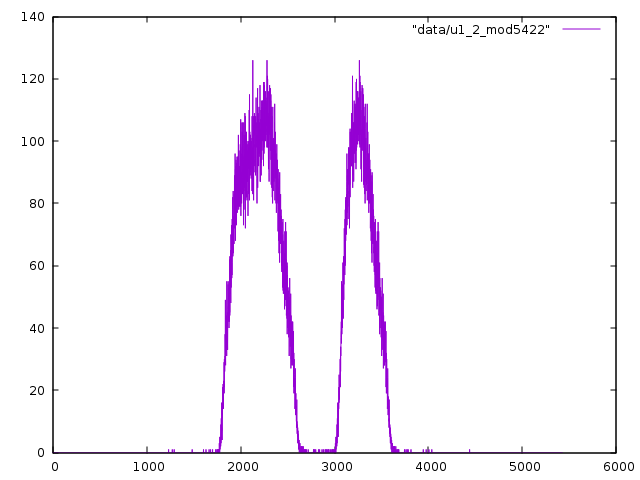
\includegraphics[scale=0.5]{../figs/u1_2_mod5422.png}

This has some notable features: 

\begin{itemize}
\item From the value of $\widehat{1_A}(0)$, it looks like the Ulam
  sequence has small but nonzero density (in fact, around $0.07$).

\item As noted in \cite{ulam_steinerberger} it looks like as we increase $N$
  that this is converging to an actually continuous distribution.

\item It looks at a glance like this distribution is supported on the
  middle third of the interval $[0,\frac1\alpha]$.  This is not
  literally the case, but in \cite{avoid_zero_gibbs} there is a
  conjecture in this direction.

\end{itemize}

{\color{red}

TODO: More questions--do the easy-to-explain-now highlights of the
later ``Questions'' section.

\subsection{Results}

TODO: Highlight the major results (whatever those end up being)

}
\section{Background}

We will start by giving an overview of some known results that should
lead us in the right direction.  No arguments in this section are
original unless noted otherwise.

\subsection{Known regularity results}

If we want to prove this kind of generalised regularity statement, it
might help to understand existing proofs of regularity (i.e. that
consecutive differences are eventually periodic).  We discuss two such
results in this section.

\subsubsection{Finch's criterion for regularity}

In \cite{regularity_criterion_finch}, Finch proves:

\begin{theorem}
If $A = U(a,b)$ is a 1-additive set containing finitely many even
elements, then $A$ is regular.  
\end{theorem}

The idea of the proof is that if there are finitely many evens, say
$e_1 < \ldots < e_s$, then every term $n$ after the last even must be
odd.  Since it can be written as sum of two earlier terms, and it is
odd, one of its summands must be even.  And since it can be written in
such a sum in a unique way, this is saying that $n - e_i$ is in the
sequence for a unique $i$ from 1 to $s$.  This is finitely many things
to check.

More precisely:

\begin{proof}

  If $x_n$ is the number of representations of $n$ as a sum of two
  elements of $A$ and $n$ is odd, then because an odd number that is a
  sum of two smaller elements of $A$ must have an even summand and we
  have only finitely many evens $e_1 < \ldots < e_s$, we can write a
  finite recurrence:

  \[x_n = \sum_{i=1}^s 1(x_{n-e_i})\]
  
  where $1(x)$ is 0 unless $x = 1$, in which case $1(x) = 1$.  In
  particular, $0 < x_n \leq s$ for all odd $n > e_s$.  Note also that
  $x_n$ depends on a finite range of earlier $x_i$'s:
  $x_{n-2}, x_{n-4}, \ldots, x_{n-e_s}$.  Call this sequence $B_n$.
  Each of the $e_s/2$ values in $B_n$ is between 1 and $s$, so there
  are finitely many possible such sequences.  Thus, for some $N$ and
  $n$, we must have $B_n = B_{n+N}$.  But since $x_n$ and $x_{n+N}$
  only depend on $B_n$ and $B_{n+N}$ respectively, this means
  $x_n = x_{n+N}$.

  And further, $x_{n+2}$ and $x_{n+N+2}$ only depend on the sequences
  $B_{n+2}$ and $B_{n+N+2}$, respectively.  But 

  \begin{eqnarray*}
    B_{n+N+2} &=& (x_{n+N}, x_{n+N-2}, \ldots, x_{n+N+2-e_s}) \text{
    by definition}\\
    &=& (x_{n+N}, x_{n-2}, \ldots, x_{n+2-e_s}) \text{ because $B_n
                                                  = B_{n+N}$}\\
    &=& (x_{n}, x_{n-2}, \ldots, x_{n+2-e_s}) \text{ as noted
                                                above}\\
              &=& B_{n+2}\\
  \end{eqnarray*}

  So in fact $B_{n+N+2} = B_{n+2}$ and we can proceed by induction to
  show the $B_n$ are periodic with period $N$.  Since the $x_n$ are a
  function of the $B_n$, $x_n$ is therefore also periodic with period
  $N$.
\end{proof}

Using empirical computations inspired by this criterion, Finch
conjectures \cite{patterns_finch} that the following is the complete
list of $(a,b)$ with $U(a,b)$ regular:

\begin{conjecture}[Finch]
  $U(a,b)$ has only finitely many even terms if and only if $(a,b)$ is
  in the following list:

\begin{itemize}
\item $(2,v)$ for $v \geq 5$ and odd.
\item $(5,6)$.
\item $(u,v)$ for $u \geq 4$ and even.
\item $(u,v)$ for $u \geq 7$ and odd if $v$ is even.
\end{itemize}
\end{conjecture}

In particular the conjecture implies that all of these sequences are
regular, although it may not be the complete list of regular $U(a,b)$.

\subsubsection{Regularity of $U(2,2n+3)$}

Using the above criterion, Schmerl and Speigel in
\cite{regularity_schmerl} prove: regularity for the 1-additive sets
$U(2, 2n+3)$:

\begin{theorem}
The 1-additive sets $U(2,v)$ for $v > 5$ and odd are regular.
\end{theorem}

Since they use Finch's criterion, this boils down to showing that each
of these sets has finitely many evens.  Specifically: 

\begin{lemma}The only even elements in the 1-additive set $U(2,v)$
  (with $v > 5$ odd) are 2 and $2v+2$.
\end{lemma}


\begin{proof}
  The proof goes by supposing that $x$ is the next even element of
  $U(2,v)$ after $2v+2$ and using an exhaustive knowledge of small
  elements of the sequence (up to about $5v$) to write $x = a+b$ for
  smaller $a, b \in U(2,v)$ in more than one way.  To do this, we have
  to understand the small elements of the sequence and the elements
  just before $x$.  

  We leave out the computation of the small elements and simply state
  the result: 

  \begin{lemma}
    The elements of $U(2,v)$ up to $5v+10$ are: 

    \begin{itemize}
      \item $2$
      \item $2v+2$
      \item All odds between $v$ and $3v$, inclusive.
      \item $3v+4i$ for $0 < i \leq \frac{v+1}{2}$ (that is, every
        other odd from $3v$ to $5v+2$ inclusive)
      \item $5v+4$
      \item $5v+10$
    \end{itemize}
  \end{lemma}

  To use these to express our supposed next even element $x$ as a sum
  of elements of $U(2,v)$ in multiple ways, we also need to understand
  the elements immediately leading up to $x$.  

  \begin{lemma}
    There is no gap of length $2v$ in the odd numbers in the sequence
    up to $x-2v$.  More precisely, if $r$ is any odd number less than
    $x-2v$, then one of $r, r+2, \ldots, r+2v$ is in $U(2,v)$.  
  \end{lemma}
  \begin{proof}
    If we take $r$ to be the minimal counterexample to this, then $r-2$
    is in $U(2,v)$, else $r-2$ would be a smaller counterexample (note
    that 1 is manifestly not a counterexample, so $r-2 > 0$).  

    But then $r+2v = (r-2)+(2v+2)$ expresses $r+2v$ as a sum of
    elements of $U(2,v)$, so the only way it can fail to be in
    $U(2,v)$ is if there is another such expression.  But $r+2v$ is
    odd, so any other expression of it as $a+b$ for $a, b \in U(2,v)$
    requires that one of $a$ and $b$ be even.  And $r+2v < x$, so the
    only choice other than $2v+2$ (which we have already used) is 2.
    So this means $r+2v = 2+(r+2v-2)$ is the other such expression.
    But for this to be such an expression, $r+2v-2$ must be in
    $U(2,v)$, and we are done.
  \end{proof}

  \begin{corollary}
    It follows from the proof that for any odd $r < x-2v$
    $r \in U(2,v)$ if and only if exactly one of $r+2v+2$ and $r+2v$
    is in $U(2,v)$.
  \end{corollary}

  This will allow us to, for example, find several elements of
  $U(2,v)$ between $x-3v$ and $x$.  We already know that we have a lot
  of elements between $v$ and $3v$, so this gives us a good chance of
  expressing $x$ as a sum of elements of $U(2,v)$ in multiple ways.  

  For example, the second lemma tells us that some odd between $x-3v$
  and $x-v$, say $x-v-2i$ (for some $0 \leq i \leq v$) is in
  $U(2,v)$.  But we know everything of the form $v+2i$ with $0 \leq i
  \leq v$ is in $U(2,v)$ as well, so: 

  \[x = (x-v-2i)+(v+2i)\]

  is the qualifying expression for $x$ as a sum of smaller elements.
  Since this expression must be unique, we also know that $x-v-2j$ for
  $0 \leq j \leq v$ and $j \neq i$ cannot be in $U(2,v)$.  

  To get a second such expression (and therefore a contradiction), we
  will look also at the odd elements from $x-5v$ to $x-3v$, using our
  knowledge of the odd elements of $U(2,v)$ from $3v$ to $5v$.  

  After some casework, this will end up giving a second qualifying
  expression for $x$, thereby disqualifying it.  We refer to
  \cite{regularity_schmerl} for the details.
  
  % We shall look at these elements by considering
  % $y_k = (x-v-2k) - (2v+2)$.  By the corollary, $y_k$ is in $U(2,v)$
  % if and only if exactly one of $y_k+2v+2 = x-v-2k$ and
  % $y_k+2v = x-v-2(k+1)$ is in.  But this only happens if $k = i$ or
  % $k+1=i$, so the only elements in $x-3v$ to $x-5v$ that are in
  % $U(2,v)$ are $x-3v-2i-2$ and $x-3v-2i$.  

  \end{proof}

\subsection{Sum-free sets}

The set of Ulam numbers $A$ has the property that for each $a \in A$,
there is exactly one solution to $x+y=a$ with $x < y$ in $A$.  The
condition that $x < y$ is a little hard to capture using standard
techniques, but, for example, this entails that the number of
solutions to $x + y = a$ with $x, y \in A$ is at most 3 (namely, the
unique solution $x+y = a$ above, then also $y+x = a$, and then
possibly some other $z+z = a$, since the definition of the Ulam
numbers does not consider this.  For example, 4 is Ulam, and its
unique representation is $1+3=4$, but it also happens that $2+2=4$ and
2 is also Ulam).

In particular, this implies that if $A_N$ is again the set of Ulam
numbers up to $N$, then $A_N$ has at most $3|A_N|$ solutions to $x+y =
z$ with $x, y, z \in A_N$.  

We might ask how special such a condition is on sets of integers.  For
instance, suppose we take the integers up to $N$ and we generate a
random subset by including each one with probability $p$.  The size of
set we expect to get is $pN$.  The number of pairs $x,y$ is $(pN)^2$,
and of these, we expect $p$ of them have $x+y$ in the set, so we
expect $p^3 N^2$ solutions to $x+y=z$.  In particular, an arbitrary
set of density $p$ we expect to have $O(N^2)$ solutions.  Since the
Ulam numbers appear to have density around $0.07$ but by construction
have only $O(N)$ solutions to $x+y=z$, they are already somewhat
special.  

In the interest of understanding what precisely is happening with the
Ulam numbers, then, we might turn our attention to the more extreme
situation of sets with no solutions to this equation at all: So-called
``sum-free sets''.  

\begin{definition}
  A subset $A$ of an abelian group is \textbf{sum-free} if the
  equation $x+y=z$ has no solutions with $x, y, z \in A$.
\end{definition}

\begin{example}
\begin{enumerate}
\item The odd positive integers are sum-free.  
\item More generally, if $A \subset \Z/m$ is sum-free, then the set of
  integers $x$ that reduce to an element of $A$ modulo $m$ is also
  sum-free.  
\item Even more generally, for any homomorphism $\pi : \Z \to \R/\Z$,
  if $A$ is a sum-free subset of $\R/\Z$, then $\pi\inv(A)$ is a
  sum-free set of integers.
\item Any subset of a sum-free set is sum-free also.
\end{enumerate}
\end{example}

When we think about generalising the particular notion of
``regularity'' above for the purpose of the Ulam sequence or for
sum-free sets, the basic idea is that a set should be ``regular'' if
it has some correlation with a set of the form in example 3.

\subsubsection{Decision sequences}

It turns out there is a construction that bijects sum-free sets of
positive integers with infinite binary sequences.  In words, the
construction is simple: Take the positive integers in turn starting
with 1.  Flip a coin.  If it's heads, include it in the set and erase
all integers that are sums of elements in the set thus far (as these
could not be in the set if it is to be sum-free).  If tails, do not
include that integer in the set.  Then move on to the next integer
that has not been included, excluded, or disqualified.

More formally: 

\begin{definition}Define the function
  $\theta : \{0,1\}^\N \to \{f : \N \to \{0,1\}\}$ from binary
  sequences to sum-free sets of natural numbers (or, in this case,
  their indicator functions) as follows: If $s\in\{0,1\}$ is a binary
  sequence, then using $s$, we will actually define three disjoint
  sets that partition the natural numbers: The target set $A$, the
  excluded set $E$, and the disqualified set $D$.  For each
  $n \in \N$, iteratively select a set for $n$ as follows:

\[\begin{cases}
n \in A+A &\implies n \in D\\
n \notin A+A \text{ and } s_k = 1 &\implies n \in A\\
n \notin A+A \text{ and } s_k = 0 &\implies n \in E
\end{cases}\]

where, at each stage, $k = |A|+|E|+1$ is the index of the first
element of $s$ that we have yet to consult. 

If $S$ is a sequence and $A$ is a sum-free set with $\theta(S) = A$,
then $S$ is called the \textbf{decision sequence} for $A$.
\end{definition}

\begin{example}
  For example, let us compute $\theta(111111111...)$: We start with 1
  and flip a coin and get heads, so we include 1 in the set $A$.  This
  automatically disqualifies 2 as $2 = 1+1$.  The next possible
  candidate is 3, so we flip another coin and get heads, and so we
  include 3.  This automatically disqualifies 4 ($4 = 1+3$) and 6
  ($6 = 3+3$).  Continuing in this way, it is clear we will never get
  a chance to include an even number and will always include the odd
  numbers, so in the end, the result is the set of odd positive
  integers.
\end{example}

It is also possible to reverse this construction.  In words: Say we
start with $A$ a sum-free set.  We again walk through the positive
integers starting at 1.  For each $n$ there are three possibilities:
Either $n \in A$, $n \in A+A$, or neither.  If $n \in A$, then it got
there by a coin landing heads, so we write down a 1.  If $n \in A+A$,
then $n$ was disqualified from being in $A$ not by a coin flip, but by
being a sum of elements of $A$, so we write down nothing.  If $n
\notin A$ and also $n \notin A+A$ then $n$ could have been included in
$A$, but was excluded simply because of a coin flip, so we write down
a 0.  

Formally, we write down the sequence $s = \theta\inv(A)$ by writing
down first the string $s'$ whose $n$th character is: 

\[s'_n = \begin{cases}
\text{`A'}& \text{if } n \in A\\
\text{`D'}& \text{if } n \in A+A\\
\text{`E'}& \text{if } n \notin A \cup (A+A)
\end{cases}\]

(So all the `A's are elements of $A$, all the `D's are automatically
excluded from $A$ by being sums of prior elements of $A$, and all the
`E's are things that are excluded from $A$ despite the fact that their
inclusion would not violate the sum-free property.)  Then the decision
sequence $s$ of $A$ is got by starting with $s'$ and deleting all
$D$s, replacing all $A$s with 1, and replacing all $E$s with 0.

There are many questions about this construction.  For example, it is
known that if a sum-free set $A$ is regular (as defined
above--i.e. its sequence of successive differences is ultimately
periodic), then its decision sequence $\theta\inv(A)$ must also be
ultimately periodic \cite{sumfree_cameron}.  The converse is believed
to be false, with one of the simplest apparent counterexamples being
$\theta(\overline{01001})$ ($\overline{01001}$ meaning the binary
sequence that repeats the pattern $01001$ forever).  This is a set
$\{2, 6, 9, 14, 19, 26, 29, 36, 39, 47, 54, 64, 69, 79, 84, 91, 96,
\ldots\}$ that has been computed extensively and for which no period
has been identified.  There is other computational evidence that this
sequence may not be periodic beyond just brute force attempts to
compute a period found in \cite{difference_density_calkin}.
Nevertheless, there is no known example of an ultimately periodic
decision sequence for which we can prove its corresponding sum-free
set is non-regular.

\subsubsection{Density and regularity}

We start with the observation that if $A$ is a sum-free set and
$a \in A$, then $A$ and $A+a$ are disjoint sets of integers.  This
automatically guarantees that a sum-free set cannot have density in
the integers of more than $\frac12$.  Specifically: 

\begin{definition}
  A subset $A \subset \Z^+$ has \textbf{density} $\delta$ if
  $\lim_{N \to \infty} \frac{|A_N|}{N}$ exists and is equal to
  $\delta$.
\end{definition}

Since this may not always exist, we might work with another number
that always will exist and that, in cases when the density does not
exist, provides what should be thought of as at least an upper bound: 

\begin{definition}
  A subset $A \subset \Z^+$ has \textbf{upper density} $\delta$ if
  $\limsup_{N \to \infty}\frac{|A_N|}{N} = \delta$.
\end{definition}

As we have noted, then, the maximal upper density a sum-free set can
have is $\frac12$, which is realised by the example of the odd
positive integers.  Luczak has given a sort of converse to this
example, proving in \cite{sumfree_regularity_luczak} the following: 

\begin{theorem}[Luczak]
If $A$ is a sum-free set of positive integers and there is at least
one even integer in $A$, then the upper density of $A$ is bounded
above by $\frac25$.  
\end{theorem}  

The proof is short, but a
little delicate, and we shall recall a version of it in this section.

The basic idea of the proof is to find disjoint subsets of $[N]$ that
are the same size as $A_N$, or of a size related to $A_N$.  For
example, if $a \in A_N$ is any element, then because $A$ is sum-free,
$A_N$ and $A_N+a$ are disjoint in $[N+a]$, but have the same size, and
thus $2|A_N| \leq N+a$, i.e. $|A_N|/N \leq \frac12 + \frac{a}{2N}$.
Taking the limit as $N \to \infty$, we again deduce our earlier
statement about $A$ having density bounded by $\frac12$.

\begin{proof}
Note first that if $A$ is all even elements, then $\frac12 A$ is
also sum-free, and therefore with density $\leq \frac12$, and so $A$
has density $\leq \frac14$ and the result is automatic, so without
loss we may assume $A$ has at least one odd element in addition to its
at least one even element.  

With this in mind, the proof breaks up into two cases: Where $A$
contains consecutive elements and where it does not.

\textbf{Case 1: $A$ has no consecutive elements} In the case where $A$
has an even element but no two consecutive elements, let $t$ be the
minimal odd positive element of $A-A$ which does exist using the odd
and even elements, and is not 1, since there are no consecutive
elements.  Also fix $x, y \in A$ with $t = x-y$.

This means that if $a \in A$, then $a+t-2$ cannot be in $A$ (else
$t-2$ would be a smaller odd positive difference than the minimal odd
difference $t$).  Put another way, if $a$ and $a+2$ are both in $A$,
then $a+t$ cannot be in $A$.  Put another way, if $B$ is the set of
$a \in A$ with $a+2$ also in $A$, then $B+t$ and $A$ are disjoint.  Of
course, we already know that finding two disjoint subsets of size even
as large as $|A|$ is already easy, however this lets us in fact find
three: Since $t=x-y$, this means $B+x-y$ and $A$ are disjoint, meaning
$B+x$ and $A+y$ are disjoint.  But both of these are contained in
$A+A$, so they are both also disjoint from $A$.  Thus we have $A$,
$A+y$, and $B+x$ all disjoint.  If we truncate $A$ to $A_N$, then
these are all disjoint subsets of $[N+x]$, and so

\[2|A_N|+|B_N| \leq N+x\].

So if we can relate $|B|$ to $|A|$ (for the moment using the shorthand
$B = B_N$, $A = A_N$), then we are done.  

But by the definition of $B$, we have two cases for an element of $A$: 
\begin{itemize}
\item $a \in B$, in which case $a+1$ is not in $A$.  
\item $a \in A\setminus B$, in which case we know $a+1$ is not in $A$
  (since $A$ has no consecutive elements) and $a+2$ is not in $A$,
  (since otherwise $a$ would be in $B$).
\end{itemize}

So we have the five sets:
$B, B+1, A\setminus B, A\setminus B + 1, A\setminus B + 2$, and these
are all pairwise disjoint in $[N+2]$.  (The only one that might not be
clear is $B+1 \cap A \setminus B + 2$, but if $a \in A\setminus B$ and
$b \in B$ with $a+2=b+1$, then $a + 1 = b$, giving two consecutive
elements of $A$ which does not happen.)

Thus $2|B_N| + 3(|A_N| - |B_N|) \leq N+2$, i.e.

\[|B_N| \geq 3|A_N| - N - 2\]

Now we have a relationship between $|B|$ and $|A|$, so we can pair
this with our earlier inequality relating the two of them to $N$ and
find:

\[2|A_N| + 3|A_N| - N - 2 \leq N+x \]

or
 
\[\frac{|A_N|}{N} \leq \frac25+o(1) \]

as we wanted.

\textbf{Case 2: $A$ has consecutive elements:} In the case where $A$
has $d$ consecutive elements $a, a+1, \ldots, a+d-1$, say, the
argument is similar in flavour to the above, but the technical details
are all slightly different.  We will first need a $t$ to serve the
role of our $t$ in case 1.  But now, the minimal odd difference is
simply 1.  So we do something slightly different: This time, we let
$t$ be any positive element of $A-A$ for which $t+1, \ldots, t+d$ are
all not in $A-A$.  

\begin{lemma}Such $t$ does exist\end{lemma}

\begin{proof}Since $a, a+1 \in A$, we know $1 \in A-A$.  Then let $t$
  be the maximum of $1, \ldots, a-1$ that is in $A-A$, so nothing from
  $t$ to $a-1$ is in $A-A$ (by definition), and nothing from $a$ to
  $a+d-1$ is in $A-A$ either (since these are all in $A$), so at least
  $d$ elements (and possibly more) immediately after $t$ are not in
  $A-A$).
\end{proof}

Again, write $t = x-y$ for some fixed $x, y \in A$.

We proceed broadly as before on the two-step plan: 

\begin{enumerate}
\item Find a set $B$ of elements that gives rise to many disjoint
  subsets of $[N]$ and deduce a bound relating $|A_N|$ and $|B_N|$ to
  $N$.
\item Upper-bound $|B_N|$ in terms of $|A_N|$ and $N$, and plug this
  into the previous bound to get a bound on $|A_N|$ in terms of $N$.
\end{enumerate}

\textbf{Step 1: }Let $B$ be the set of elements $b$ for which
$b+1, \ldots, b+d-1$ are all not in $A$.  Then certainly the sets
$A, B+1, \ldots, B+d-1$, are all disjoint.  In fact, we can get one
more than this: We can shift all these sets by $a$ and they are still
disjoint: $A+a, B+a+j$ ($j=1, \ldots, d-1$).  But now since the $a+j$
are all in $A$, these sets are all themselves disjoint from $A$ (since
they are all subsets of $A+A$).  Thus, again truncating at $N$, we
have two sets of size $|A_N|$ and $d-1$ sets of size $|B_N|$ all
disjoint and inside $[N+a+d-1]$.  Thus:

\[2|A_N|+(d-1)|B_N| \leq N+a+d-1\]

\textbf{Step 2: }So again, we need control over the size of $|B_N|$ in
terms of $|A_N|$ and we will be done.  But this time, we note that if
$z \in A$, it is possible that $z+t$ could be in $A$, but that then
because of the definition of $t$, none of $z+t+1, \ldots, z+t+(d-1)$
can be in $A$ (lest one of $t+1, \ldots, t+(d-1)$ lie in $A-A$).  Thus
elements of $A+t$ that lie in $A$ in fact must lie in $B$.  Put another
way, $A+t$ and $A \setminus B$ are disjoint.  Again, this is only two
sets, but we can use the same trick as before to make it three: Since
$t = x-y$, we can equally say $A+x$ and $(A \setminus B) + y$ are
disjoint, at which point these are also disjoint from $A$ (again,
being subsets of $A+A$).  So we have three disjoint subsets $A+x$,
$A \setminus B + y$, and $A$ of $[N+x]$, with sizes $|A_N|$, $|A_N|$,
and $|A_N|-|B_N|$, respectively.  This gives
$|A_N| + |A_N| + (|A_N| - |B_N|) \leq N+x$ or:

\[|B_N| \geq 3|A_N|-N-x\]

Dropping this into the first inequality and rearranging, we get:

\[2|A_N|+(d-1)(3|A_N|-N-x) \leq N+a+d-\]

which simplifies to: 

\[\frac{|A_N|}{N} \leq \frac{d}{3d-1} + o(1)\]

Since $d \geq 2$ (as we are assuming we have at least two consecutive
elements), this is again bounded by $\frac25$ in the limit, so the
claimed bound follows.
\end{proof}

\subsubsection{Aperiodic sum-free sets}

A construction of Erdos in \cite{aperiodic_sumfree_erdos} supplies an
example of a sum-free set with density $\frac13$ that has no
periodicity, namely: Take $\alpha \in \R$ irrational, and let
$A_\alpha$ be the set of integers $n$ such that $n \mod{\alpha}$ lies
in $\left(\frac \alpha 3, \frac {2\alpha}{3}\right)$.  $A_\alpha$ is
clearly sum-free, since it is sum-free modulo $\alpha$, but for
irrational $\alpha$, $A_\alpha$ is also not periodic.  That is, for
every modulus $m$ and every residue class $k$, there is an element of
$A_\alpha$ congruent to $k$ mod $m$.  

Indeed, equidistribution results for irrational numbers tell us that
there the integers are equidistributed modulo any irrational.  For
example, there is at least one $n$ that reduces to the interval
$\left(\frac{\alpha}{3m}-k,\frac{2\alpha}{3m}-k\right)$ modulo the
irrational number $\frac{\alpha}{m}$.  Then it is clear that $mn+k$
will reduce to $\left(\frac{\alpha}{3},\frac{2\alpha}{3}\right)$ mod
$\alpha$, meaning that $mn+k \in A_\alpha$ as desired.
{\color{red}

\subsection{Abelian arithmetic regularity}

% If $A$ is any set, then an easy probablistic argument shows that there
% is a sum-free subset of $A$ of size $|A|/3$.  Indeed, if for any real $\alpha$,
% we define $A_\alpha$ to be set the set of elements $x$ of $A$ with

% \[A_\alpha = \{x \in A : 1/3 < \alpha x \mod{1} \leq 2/3\]

% then the expected size of $A_\alpha$ is $|A|/3$ as $\alpha$ varies
% over $[0,1]$, and so there must be at least one a for which $A_\alpha$
% has at least this size.

% In \cite{no_large_sumfree_subset_eberhard} prove that for every e > 0, there is a set A such
% that A has no sum-free set larger than $(1/3 + \epsilon)|A|$, so this
% bound is in fact sharp (to first order).  (Apropos of nothing, I find
% this paper's organisation and general exposition to be highly
% user-friendly and otherwise excellent.)

% In our case, if $A$ is the Ulam sequence up to N, then for any
% $\epsilon > 0$ we believe that for $N$ large enough, we could generate
% a sum-free subset of size $(1-\epsilon)|A|$--kind of the opposite
% extreme.

% Nevertheless, the argument follows a kind of local-to-global flow that
% might make it worth understanding, so we work through at least the
% basic idea here:

% ...

}

\subsection{Roth's theorem}

Roth's theorem is about the number 3-term arithmetic progressions
$x, y, z$ in a set $A \subseteq \Z^+$.  Specifically: 


\begin{theorem}[Roth's theorem]
  Let $A \subseteq Z^+$ be a set of positive integers with positive
  upper density.  Then $A$ contains infinitely many arithmetic
  progressions $a, a+d, a+2d$ of length 3.  
\end{theorem}

Equivalently, such an $A$ always has at least one solution to $x+z=2y$
(whereupon $x, y, z$ is an arithmetic progression of length $3$).  A
sum-free set $A$ instead has are no solutions to $x+z=y$ (swapping
around variable names to highlight the similarity), so if we have a
sum-free set that we believe has positive density, we might wonder
what the proof of Roth's theorem has to say about it.  (After all, in
the case of the slightly different equation $x+z=2y$ it says that the
set $A$ cannot exist.)

As it turns out, many new techniques in additive combinatorics cut
their teeth on Roth's theorem, and so there are many proofs, from
those that use probabilistic techniques to ergodic theory.  We will
discuss two in particular: The density increment and energy increment
proofs.  We will not give the complete proofs in either case, but will
simply work through the steps that we shall return to later and
outline the rest.

\subsubsection{Density increment proof}

Proofs of Roth's theorem often work with a finitary version of the
statement, which we make now:

\begin{theorem}[Roth's theorem]
  For every $\delta > 0$, there is an $N_0 > 0$ such that for every
  $N > N_0$, every $A \subseteq [N]$ with $|A| > \delta N$ contains a
  solution to $x+z=2y$.
\end{theorem}

One strategy of proof goes via Fourier analysis, saying that if $A$
has no large Fourier coefficients, then $A$ is guaranteed to behave
``pseudorandomly'' in some sense, and computes that such sets must
automatically have many length-3 arithmetic progressions, and we are
done already.  

If, on the other hand, $A$ does have some large Fourier coefficient,
then one can find a long arithmetic progression that has large
intersection with $A$, and on which $A$ in fact has higher density
than it had originally.  We can repeat this step (the ``density
increment'') as often as needed until either our intersected $A$ has
no large Fourier coefficient (in which case we are done as above) or
else $A$'s density in the arithmetic progression increases to 1.  If
we are careful about it, we can ensure that at least 3 elements will
still remain by the time we get to this point.

\begin{proof}[Proof of Roth's theorem via density increment]

  Rather than working on the set $[N]$, we shall work with the group
  $\Z/N$, noting that if $A$ only contains elements smaller than
  $N/2$, then a solution to $x+z=2y$ in $\Z/N$ is an honest solution
  to $x+z=2y$ in $A$ viewed as a subset of $\Z$.  

  If $A$ is a set of density $\delta$ in $\Z/N$, then the number $S$
  of solutions to $x+z=2y$ is counted by

  \begin{eqnarray*}
    S &=& \frac1N \sum_{t=0}^{N-1} \hat 1_A(t)\hat 1_gA(t)\hat 1_A(-2t) \\
    S &=& \frac1N |A|^3 + \frac1N \sum_{t=1}^{N-1} \hat 1_A(t)\hat 1_gA(t)\hat 1_A(-2t) \\
      &=& \delta^3 N^2 + \frac1N \sum_{t=0}^{N-1} \hat 1_A(t)^2\hat 1_A(-2t) \\
      &\geq& \delta^3 N^2 - \sup_t |\hat 1_A(-2t)| \frac1N \sum_{t=0}^{N-1} |\hat 1_A(t)|^2 \\
      &=& \delta^3 N^2 - \sup_t |\hat 1_A(-2t)| \frac1N \sum_{t=0}^{N-1} |1_A(t)|^2 \\
      &=& \delta^3 N^2 - \sup_t |\hat 1_A(-2t)| |A|\\
      &=& \delta^3 N^2 - \sup_k |\hat 1_A(k)| \delta N
  \end{eqnarray*}

  So if there is no large Fourier coefficient--that is, every Fourier
  coefficient is $\leq \epsilon N$, then
  
  \[S \geq (\delta^3 - \delta\epsilon) N^2\]

  So if $\epsilon < \delta^2$, then $S > 0$, at which point there is at
  lest one solution, as desired.  
  
  If, on the other hand, there is a $k$ such that
  $|\hat 1_A(k)| \geq \delta^2 N$, then this argument does not
  guarantee a solution.  However, in that case, let $P = d[1,L]$ be
  the arithmetic progression of length$L$ and difference $d$
  $\{d, 2d, \ldots ,Ld\}$ ($d$ to be chosen later).  We want an
  arithmetic progression in which $A$ has higher density than it has
  in $\Z/N$ at large.  In other words, we want to find an $a$ that
  makes $Q(a) = |A \cap (P+a)| = 1_A \star 1_P(a)$ large.  But this we
  can analyse using Fourier analysis:
  
  \begin{eqnarray*}
    \hat Q(s) = \hat 1_A(s) \overline{\hat 1_P(s)}
  \end{eqnarray*}
  
  Further, we know that for all $s \neq 0$,
  $\sum_a Q(a) \geq |\hat Q(s)|$ (looking at the definition of the
  Fourier transform and using the triangle inequality).  So in
  particular, for $s = k$ (the large Fourier coefficient):

\begin{eqnarray*}
  \sum_a Q(a) &\geq& |\hat Q(k)| \\
              &=& |\hat 1_A(k)| |\hat 1_P(k)| \\
              &\geq& \epsilon N |\hat 1_P(k)| 
\end{eqnarray*}

Thus for some $a$, $Q(a)/N \geq \delta^2 |\hat 1_P(k)|$.  We can
select $d$ and $L$ such that $|\hat 1_P(k)| \geq L/2$, so for some
$A$, $Q(a)/N \geq \epsilon L/2$.  In particular, $A$ intersected with
an arithmetic progression of length $L$ has density
$\delta + \epsilon/2$, meaning we have increased the density,
whereupon we can repeat the argument.

The details (such as actually selecting the correct $d$ and $L$, as
well as properly transitioning from $\Z/N$ back to $\Z$), are covered
in many places, for example \cite{lyall_roth}.

\end{proof}

{\color{red}

\subsubsection{Proof via the regularity theorem}

The density increment proof exemplifies a kind of dichootomy between
structure and randomness in its two cases: Where $A$ behaves
pseudorandomly, in which density controls all the counting
expressions, and where $A$ has structure, which we can use exploit to
iterate the argument.

The pseudorandomness argument will carry over nicely to the sum-free
and Ulam cases, but second part of the argument relies on the fact
that the structure of interest--in the case of Roth, arithmetic
progressions, and in our case, additive triangles--can be found
equally in any arithmetic progression.  For progressions, this is
clear, but for triangles, this is simply false: The very dense
progression of all odd numbers already contains zero additive
triangles.  

As this part of the proof seems unlikely to generalise to our
situation, we explore a second avenue of proof for Roth's theorem,
namely using the arithmetic regularity and counting lemmas of the
earlier section.  This comes from \cite{higher_fourier_analysis_tao}

\begin{proof}[Proof of Roth's theorem via arithmetic regularity]
  For a function $f : [N] \to \{0,1\}$, define
  $T(f) = \sum_{x,y \in [N]} f(x)f(x+y)f(x+2y)$ to be the function
  that counts 3-term progressions if $f$ is thought of as an indicator
  function.  So our goal is to prove that for $A \subseteq [N]$ of
  density $\delta$ (for $N$ sufficiently large relative to $\delta$)
  that $T(1_A) > 0$.  
  
  As in the statement of the regularity lemma, write
  $1_A = f_{str} + f_{sml} + f_{unf}$ with parameters $M$ and
  $\epsilon$.  .
\end{proof}

%\subsection{Green's arithmetic triangle removal theorem}
}
\subsection{Quantitative bounds in finite fields}

There have been several recent developments in a finite field setting
on analogous problems (specifically, the work of Croot, Lev, and Pach
\cite{progressions_croot} on length-3 arithmetic progression-free sets
in $\FF_4^n$ and subsequent work by others \cite{capset_ellenberg}
pushing it to $\FF_3^n$.

We will recall the method used here by outlining the proof in
\cite{capset_ellenberg}, in view of the possibility of later asking
about Ulam-like sequences in the same context.

\begin{theorem}[Ellenberg-Gijswijt]
Let $\alpha, \beta, \gamma$ be elements of $\FF_q$ such that
$\alpha+\beta+\gamma = 0$ and $\gamma \neq 0$.  Let $A$ be a subset of
$\FF_q^n$ such that the equation $\alpha a_1 + \beta a_2 + \gamma a_3
= 0$ has no solutions $(a_1, a_2, a_3) \in A^3$ apart from $a_1 = a_2
= a_3$.  Then $|A| = o(2.756^n)$.
\end{theorem}

\begin{proof}Let $S^d$ be the space of all polynomial functions on
  $\FF_q^n$ of degree $d$ (that is, polynomials of total degree $d$
  where each of the $n$ variables shows up with degree less than $q$).
  Let $m_d$ be the dimension of this space, and let $V_d$ be the
  subspace of polynomial functions vanishing on the complement of $2A$
  (this is more or less a trick).  Then

  \[\dim(V_d) >= m_d - (q^n - |A|)\]
  
  (since the requirement to vanish on the complement of $2A$ is at most
  $q^n - |A|$ conditions).
  
  It turns out that we can actually get a polynomial $P_d$ in $V_d$ with
  support of size exactly $\dim(V_d)$, and so this polynomial has:
  
  \[|\supp(P_d)| >= m_d - q^n + |A|\]
  
  Now for the last bit: If we have a degree-d polynomial $P$
  vanishing on the complement of $2A$, then we can form the $|A|$ by
  $|A|$ matrix $M$ whose $i,j$ entry is $P(a_i + a_j)$ where $a_i$ are
  the elements of $A$.  First of all, because for $i$ and $j$
  different, $a_i+a_j$ is never in $2A$, the off-diagonal terms all
  vanish, whereas because the diagonal terms are $P(2a_i)$, they may
  or may not vanish.
  
  
  We can brutally expand this polynomial into a sum of monomials:
  
  \[P(a_i + a_j) = \sum_{\text{monomials m,m' of degree d or less}} c_{m,m'} m(a_i) m'(a_j)\]
  
  Further, in each term at least one of m and m' has degree at most d/2, so we can sum over 
  
  \[P(a_i + a_j) = \displaystyle\sum_{\text{monomials m of degree d/2 or less}} c_{m} m(a_i) F_m(a_j) + c'_m m(a_j) G_m(a_i)\]
  
  So $M$ is a linear combiantion of $2 m_{d/2}$ matrices $(m(a_i)
  F_m(a_j))$ each of which, as the exterior product of two vectors, has
  rank 1.  Thus the rank of $M$ is at most $2 m_{d/2}$.  And since $M$ is
  diagonal, this means that in fact on $2A$, $P$ has only $2 m_{d/2}$ non-zero
  points.  So the support of $P$ is bounded above by $2 m_{d/2}$.  Since the
  support of $P_d$ was already bounded below by $m_d - q^n + |A|$ we can
  apply this argument to $P_d$ and conclude that
  
  \[2 m_{d/2} \geq m_d - q^n + |A|\]
  
  i.e.
  
  \[|A| \leq 2 m_{d/2} - m_d + q^n\]

  Choosing a particular value of d and bounding these quantities is
  all that remains.  In \cite{capset_ellenberg} they take
  $d = 2(q-1)n/3$ and use Cramer's theorem to bound $m_d$ and related
  quantities in terms of the claimed exponential.  We refer to the
  paper for details.
\end{proof}

\section{Questions and Definitions}

Bearing in mind this landscape of ideas, theorems, and techniques, we
now raise some questions in the particular context of the Ulam numbers
and related sequences, and the various phenomena that we observe
around them.  In addition, we shall give definitions in this section
to allow us to formulate our questions precisely.

\subsection{Ulam numbers and other 1-additive sequences}

\begin{definition}\label{def:ulam}
  The \textbf{Ulam sequence} starting with positive integers $a$, $b$
  is denoted $\ulam{a}{b}$ and is the sequence with $a_1 = a$,
  $a_2 = b$, and, for $n > 2$, $a_n > a_{n-1}$ is the integer satisfying:
  \begin{enumerate}
  \item 1-additivity: There is exactly one pair of $0 < i < j < n$ with $a_i + a_j = a_n$.
  \item Greediness: $a_n$ is the smallest positive integer with the above two
    properties.
\end{enumerate}

\end{definition}

One of the first questions that was asked by Ulam himself about the
Ulam sequence $\ulam{1}{2}$ was: 

\begin{question}\label{qn:density}
  Does $\ulam{1}{2}$ have positive uppper density?
\end{question}

For all examples of Ulam-like sequences where we know the answer to
this question, the way we know is by first establishing a regularity
result, at which point positive density is immediate.  Given the known
regularity results concerning 1-additive sequences, a very basic
question about the Ulam numbers then would be:

\begin{question}\label{qn:irregular}
  Can we prove the Ulam numbers are not regular (in the sense of
  definition \ref{def:regularity})?
\end{question}

Supposing we could do so, we might then ask:

\begin{question}\label{qn:regularity_def}
  Is there a notion of ``regularity'' that generalises
  \ref{def:regularity} and that captures the behaviour observed in
  \cite{ulam_steinerberger} and that we can prove?
\end{question}

Supposing that in some way Steinerberger's constant $\alpha$ will come
into this definition, we might wonder about what it is specifically:

\begin{question}\label{qn:rationality}
  Is $\alpha$ irrational?  Algebraic?  What about
  $\frac{2\pi}{\alpha}$?
\end{question}

Beyond just asking about $\alpha$, we can ask about other features of
the spectrum: 

\begin{question}\label{qn:spectrum}
  Are there other nonzero Fourier coefficients not in $\alpha\Z$?
\end{question}

\begin{question}\label{qn:decay}
  How quickly does $\widehat{1_A}(k\alpha)$ decay with $k$?
\end{question}

Moving on from $\ulam{1}{2}$, we can also ask about similar sequences: 

\begin{question}\label{qn:other_alpha}
  How does $\alpha$ behave for other non-regular-looking Ulam-like
  sequences?  For example, supposing $\alpha_n \in (0,\pi]$ is the
  maximal Fourier coefficient associated with $\ulam{1}{n}$ (supposing
  there even is a unique such Fourier coefficient), what is the
  behaviour of $\alpha_n$ as $n$ grows?
\end{question}

Separately, in light of the triangle removal lemma, there is a set of
questions we might ask regarding the additive structure of the Ulam
sequence:

\begin{question}\label{qn:ulam_sumfree}
  What is the minimal subset $X \subseteq A$ that we might remove so
  that $A$ becomes sum-free?  (For example, the set such that $X_N$ is
  minimal among all such possible $X$ for each $N$.)
\end{question}

A very similar question that gets more precisely at such a set $X$ in
terms of the actual definition of $A$: We know that each element
$a \in A$ is written uniquely as $x+y$ for $x < y$ elements of $A$.
Certainly the set $S = \{x \in A : x + y \in A\text{ for some $y > x$
  in $A$}\}$ of ``small summands'' is a candidate for such an $X$ in
the previous question, but $S$ itself might be of interest even if it
ends up not being minimal (though one might reasonably expect that it
would be).

\begin{question}\label{qn:fulcrum}
  Can we characterise the elements of $S$?  What is the growth rate of
  $|S_N|$ as $N$ grows?
\end{question}

Finally, we can ask about the distribution that Steinerberger observes
for the Ulam sequence modulo $\frac{2\pi}{\alpha}$, starting with a
question from \cite{ulam_steinerberger}: 

\begin{question}\label{qn:continuity}
  Does the distribution of $A_N$ mod $\frac{2\pi}{\alpha}$ converge to
  a continuous distribution?  More precisely, let
  $\lambda = \frac{2\pi}{\alpha}$.  Then if for each $M > 0$ we cut up
  the interval $[0,\lambda]$ into $M$ equal intervals and define a
  step function $f_{M,N}(x)$ to be the proportion of Ulam numbers up
  to $N$ that lie in the same one of the $M$ intervals as $x$, then as
  $M$ and $N$ go to infinity, does $f_{M,N}$ converge to a continuous
  function on $\R/\lambda\Z$?
\end{question}

We can ask a lot more than just about the distribution's continuity,
however.  The distributions particularly for other Ulam-like sequences
such as $U(2,3)$ look like they have some further internal structure
as a sum of perhaps smaller, more regular-looking peaks.  So we can
ask somewhat broadly about this also: 

\begin{question}\label{qn:shape}
  What gives this distribution its particular shape?  For example,
  what about the shape of the distribution can be deduced from the
  knowledge of the spectrum alone?
\end{question}

\subsection{Sum-free sets}

We start noting the same dichotomy that existed with 1-additive sets
seems present for sum-free sets as well: Many sum-free sets with
easy-to-describe decision sequences (much as the procedure for
generating Ulam numbers was in algorithmic) are provably regular, but
for some we do not know.  For instance, we might start with the
aforementioned ``smallest'' three examples: 

\begin{question}\label{qn:sumfree_regularity}
  Are any of the sets $\theta(01001), \theta(01010)$, or
  $\theta(10010)$ regular?
\end{question}

Supposing once again (as is suggested in
\cite{difference_density_calkin}) that the answer is no, we might try
to ask similar questions with the these sets:

\begin{question}\label{qn:sumfree_spectrum}
  What does the spectrum of these sets look like?  Is there a mapping
  to $\R/\Z$ under which the indicator functions of these sets
  approach continuous-looking distributions?
\end{question}

\begin{question}\label{qn:sumfree_new_regularity}
  Does whatever notion of regularity applies to the Ulam sequence
  apply here as well?
\end{question}

\begin{question}\label{qn:sumfree_density}
  What is the density of these sets?  Is there a statement relating
  the density of 1s in the decision sequence with the density of the
  resulting sum-free set?
\end{question}

In the sum-free case, the work of Luczak outlined above gives some
relationship between the regularity of a sum-free set and its density
(saying in his case that a sum-free set that contained an even number
(i.e. whose image mod 2 was everything) had density bounded by
$\frac25$--a meaningful improvement from the automatic bound of
$\frac12$ on the density of an arbitrary sum-free set.

On the other hand, the construction of Erdos tells us that there exist
-sum-free sets with density $\frac13$ whose image mod $m$, for all $m$,
is everything.  We might ask if there is any condition we can prove in
the gap between $\frac13$ and $\frac25$.  

\begin{question}\label{qn:irregularity_density}
  If $m$ is a positive integer, what is the maximal density $d_m$ of a
  sum-free set that hits every congruence class modulo $m$?
\end{question}

For example, 

\begin{itemize}
\item $d_1 = \frac12$ (upper bound is by the argument $(A + a) \cap A =
  \emptyset$ for any $a\in A$, and lower bound comes from the example
  of the odd numbers).
\item $d_2 = \frac25$ (upper bound is by
  \cite{sumfree_regularity_luczak}, and the lower bound is established
  by the example from the same paper of integers congruent to 2 or 3
  mod 5).
\item $d_3 = \frac12$ using the same argument as for $d_1$.
\item $d_4 = \frac25$ by the same argument as for $d_2$, since
  $(2+5\Z) \cup (3+5\Z)$ covers every congruence class mod 4.
\end{itemize}

Lastly, thinking back on the arithmetic regularity lemma, we consider
the decpomosition $1_A = f_{str} + f_{sml} + f_{unf}$ for $A$ the
various sum-free or nearly sum-free sets (e.g. the Ulam sequence)
under consideration.  

\begin{question}\label{qn:fourier_complexity_density}
  What can we deduce about the structured component from our knowledge
  of the structure of $A$?  For example, $f_{str}$ comes with bounded
  Fourier complexity.  How does the spectrum of $f_{str}$ relate to
  the structure and/or density of $A$?  For example, if $f_{str}$ has
  spectrum consisting of $\alpha\Z$ and $\beta\Z$ for two independent
  irrational $\alpha, \beta$, does this guarantee some bound on the
  density of $A$?  
\end{question}

\section{Strategy}

\subsection{Overview}

In this document we shall unfortunately not answer all these
questions, nor supply a complete understanding of the observed
phenomena.  We do, however, propose a strategy that we hope will lead
to such an understanding, and we shall partially execute certain
components of that strategy.

Broadly, we will first try to understand the Fourier spectrum, and
then determine what this says about the distrubution.  This happens in
four steps:

\begin{enumerate}
  \item Prove the existence of a large Fourier coefficient at
    some $\alpha$.
  \item Prove that the spectrum of $A$ is supported in $\alpha \Z$.  
  \item Prove that the Fourier coefficients $\widehat{A}(k\alpha)$
    decay fast enough as $k \to \infty$.  
  \item Deduce features of the distribution of $A$ modulo
    $2\pi/\alpha$.
\end{enumerate}

Of this programme, we will provide results in the direction of steps 1
and 4, and computational and heuristic evidence in favour of the
others.

\subsection{Outline}

Before we embark on this journey, we provide a little fuller picture
of what we intend to actually do towards each of the steps and in the
remainder of this document: 

\begin{enumerate}
\item First, we study the large Fourier coefficient $\alpha$ and
  corresponding period $\lambda = \frac{2\pi}{\alpha}$ of various Ulam
  sequences $U(a,b)$ and sum-free $\theta(s)$ (collectively,
  ``\relevant sets'').  Specifically:
  \begin{enumerate}
  \item We use a computer program to estimate the maximal Fourier
    coefficient of many such sequences.
  \item We use a computer program to compute continued fraction
    convergents and to attempt to compute minimal polynomials for
    certain $\lambda$ to understand whether they are rational or at
    least algebraic.  We also study the constraints that would be
    imposed on a $\ulam{a}{b}$ if the corresponding $\lambda$ were to
    be rational with numerator 3.
  \item We prove the existence of an $\alpha$ for \relevant sets $A$
    (truncated at $N$) at which the Fourier transform has size
    comparable to $|A_N|$.  In fact, we show that the real part of the
    Fourier transform itself must be large compared to $|A_N|$.
  \end{enumerate}

\item We then study the complete spectrum of various \relevant sets,
  specifically:
  \begin{enumerate}
  \item We then study the complete spectrum of \relevant sets $A$,
    computing via computer program any other nonzero values of the
    respective Fourier transforms.  We will find that the Fourier
    transform for the sets we consider appears to be supported only on
    $\alpha\Z$.
  \item We construct an example of a sum-free set with a Fourier
    spectrum not supported only on some $\alpha\Z$.
  \item For some \relevant sets with spectrum $\alpha\Z$, we use a
    computer to enumerate the values of $\widehat{f}(k\alpha)$ as $k$
    grows and see how these evolve.
  \item We give an argument that suggests how one might prove the
    observed decay of these values.
  \end{enumerate}

\item Having some picture of the spectrum, we will then study the
  distribution of $A$ modulo $\lambda$ and see what information we can
  deduce from the definition as well as from the spectral information
  we have gathered in the previous steps.  Specifically:
  \begin{enumerate}
  \item First the definition of such $A$ means that whether a given
    $x$ is in $A$ is controlled largely by $r_{A+A}(x)$--the number of
    representations of $x$ as a sum of elements of $A$.  So we start
    by studying the distribution of this.  We use a computer to
    generate plots of this that suggest a high degree of regularity in
    the behaviour of this function, and we show that an estimate of
    the function using the ``major arcs'' coming from the Fourier
    spectrum bear this out, which will give us at least a very
    plausible conjecture about the behaviour of this function.
  \item Having come to some understanding of $r_{A+A}$ using the
    Fourier spectrum, we will use this to attempt to deduce features
    of the distribution itself, ultimately proving a mild theorem that
    the distribution is at least non-uniform.
  \end{enumerate}

\item Finally, we will focus specifically on $\ulam{1}{2}$ and turn to
  more combinatorial analysis of the structure of the sequence.
  Specifically: 
  \begin{enumerate}
  \item By the definition of $\ulam{1}{2}$, every element of the
    sequence has a unique expression $x+y$ for $x, y \in \ulam12$,
    $x < y$.  So we might ask which $x$'s actually show up in the Ulam
    sequence.  For the provably regular Ulam sequences, the analogous
    consideration reveals that there are only finitely many values of
    $x$ that are used in forming the sequence.  In the case of
    $\ulam{1}{2}$, we observe a highly skewed distribution of the
    ``small summands'' $x$, and make similar observations about the
    distribution of $y$ that show up and about the pairs $(x, y)$ as
    well.
  \item From these observations, we will start to get a picture of
    what combinatorial phenomenon might underlie the Ulam sequence, and
    will consider the implications in particular for the density of
    the $\ulam{1}{2}$.
  \end{enumerate}
\end{enumerate}

\subsection{About the computations}

When we refer to computations done by computer, we will mention the
code that was use to execute them by referring to various programs in
the repository \cite{computations}.  In most cases, we will be
referring to the particular file \icode{/experiments.py}.  For example,
when we talk about \icode{experiment17}, we mean the function
\icode{experiment17()} in the \icode{experiments.py} file in that
repository.  Sometimes we will refer to code in other files as well
from the same repository, and will mention where the code in question
is located in each case.

\section{Spectrum}

The first three steps of our strategy are about understanding the
Fourier spectrum of the various \relevant sets under consideration.

\subsection{Large Fourier coefficient}

The initial observation of \cite{ulam_steinerberger} is that the
Fourier transform of the indicator function of $U(1,2)$ has takes a
large value at some $\alpha$.  That is,
$\widehat{A_N}(\alpha) = \frac1N \sum_{t=1}^N A(t) e^{-it\alpha}$ is
large relative to $|A_N|$.  This suggests that $t$ being in $A$ is
correlated with $t+\frac{2\pi}{\alpha} k$ being in $A$ for various
integer $k$.  In other words, $\lambda = \frac{2\pi}{\alpha}$ behaves
somewhat like a period for $A$.

\subsubsection{Computing $\alpha$}

We will start by computing this period for several $U(a,b)$ which are
not believed to be regular by virtue of having only finitely many even
numbers.  Specifically, we will look at:

\begin{itemize}
\item $(1,v)$ for $v = 2, \ldots, 10$.
\item $(2,3)$.
\item $(3,v)$ for $v = 4, \ldots, 10$, $3 \nmid v$.
\item $(5,v)$ for $v = 7, \ldots, 9$.
\end{itemize}

We do this by running \icode{experiment1} and observe: 

\begin{tabular}{|lllll|}
\hline
$a$ & $b$ & $\alpha_{a,b}$ & $\lambda_{a,b}$ & $|\widehat{1_{a,b}}(\alpha_{a,b})|$
  \csvreader{datafiles/1additive_alphas.csv}{}
  {\\\csvcoli & \csvcolii & \csvcoliii & \csvcoliv & \csvcolv}
\\\hline
\end{tabular}

Similarly, we can compute the $\alpha$ maximising
$\widehat{1_A}(\alpha)$ for various sum-free sets $A$--for example,
those that are believed to be non-periodic.  In particular, we will
look at $s = 01001, s = 01010$, and $s = 10010$ by running
\icode{experiment2}:

\begin{tabular}{|llll|}
\hline
$s$ & $\alpha_{s}$ & $\lambda_{s}$ & $|\widehat{1_s}(\alpha_{s})|$
  \csvreader{datafiles/sumfree_alphas.csv}{}
  {\\\csvcoli & \csvcolii & \csvcoliii & \csvcoliv}
\\\hline
\end{tabular}

{\color{red}
\subsubsection{Is $\alpha$ rational?  Algebraic?}

It is more likely that there is a sequence of m mod which the
congruence classes of $a_i$ are increasingly clustered.  The continued
fraction of $2\pi/\alpha$, which we're imagining is $m/k$, doesn't have some
really large coefficient where we would obviously truncate it.
Instead, for $2\pi/\alpha_{1,2}$ it is just
\[[2; 2, 3, 1, 11, 1, 1, 4, 1, 1, 7, 2, 2, 6, 5, 3, 1, 3, 1, 2, 1, 3, 2, 1, 14, 2, 5, 3, 2, 3, 1, 2, 13, 2]\]

(For most of the $\alpha_{a,b}$ that we computed to any meaningful
precision, either this "not obviously a rational number" continues to
be true, except when there is a very small obvious modulus like 2.)

This gives rational approximations: 
\[5/2, 17/7, 22/9, 259/106, 281/115, 540/221, 2441/999, 2981/1220, 5422/2219, 40935/16753, 87292/35725\]

% More possible arguing for irrationality: 


These suggest, for example, that for $m = 540$, there should be
substantial bias in which congruence classes show up in the Ulam
sequence.

This is borne out in very crude measurement by taking the first
100000 terms of the Ulam sequence and computing them mod, e.g. 540, and
asking how often each congruence class mod 540 shows up and computing
the standard deviation of all these numbers.

% 215519 & 482.8027781782595\\
% 1380406 & 304.5611017423058
% \end{tabular}

Note, however, that while it looks like the bias starts falling off at
40935, in fact we only know alpha to within $10^(-10)$ or so, and for
$p/q$ convergents from the continued fraction,
$|\alpha - p/q| < 1/q^2$.  So being confident about alpha to within
$10^{-10}$ suggests that we should only trust convergents up to 5-6
digits.

Moreover, we note that if we take fewer terms, then fewer of the terms
will be less than the modulus, so we may see less of the bias even if
there is some.  For example, the same calculation with only the first
10000 terms looks like:

\begin{tabular}{ll}
5 & 21.633307652783937\\
17 & 61.68515885956209\\
22 & 72.60478321332931\\
259 & 89.57462754381896\\
281 & 193.62880436289325\\
540 & 682.2864609640275\\
2441 & 382.62668898244124\\
2981 & 348.9472882781135\\
5422 & 263.99360062887\\
40935 & 122.81328398767178\\
87292 & 105.0829179694691\\
215519 & 97.65246431214172\\
1380406 & 99.63712935143478
\end{tabular}

Also of note is that if we repeat the computation with $N=100000$ with
other random moduli, then we don't see numbers of that magnitude at
all:

\begin{tabular}{ll}
...&...\\
538 & 266.52186279126255\\
539 & 255.35109519675422\\
540 & 664.2715810068448\\
541 & 258.6315258698218\\
542 & 263.9800814357665\\
...&...\\
2439 & 264.9962194257936\\
2440 & 255.43572224088751\\
2441 & 3022.3025069077416\\
2442 & 258.0622079927702\\
2443 & 255.08506362547774\\
...&...\\
\end{tabular}

One takeaway from this study of increasing moduli is the following:
earlier we discussed the possibility of the behaviour indicting bias
mod some m.  In fact, there may not be a single m with the most bias,
but an increasing sequence of m's with progressively more bias.  For
example, one could imagine a sequence that is slightly biased to being
odd, say 60\% are 1 mod 2.  But then in fact it turns out that mod 4,
it is more strongly biased, with 65\% being only 2 or 3 mod 4.  And
maybe in fact mod 12, 80\% of terms are only ever 2, 3, 6, or 8 mod 12,
and maybe in fact 99\% are 2, 3, 6, 8, or 1 mod 48, and maybe you can
catch more and more of the sequence with a slowly expanding set of
congruence classes modulo quickly growing modulus.  If there is a
"bias mod $m$" thing happening, this is probably the flavour it takes,
but I'm happy to try to treat the approximation to alpha as indicating
an "at least some bias toward some congruence classes mod some fixed
$m$" phenomenon.

% end possible argument

My guess is that since apparently alpha=pi sometimes, alpha should not
be expected to be algebraic, but really $2pi/alpha$ is the relevant
quantity anyways. At any rate, we tried some tests on both using LLL
to hunt for the minimal polynomial of $b = 2pi/alpha$ and b = alpha. It
should be noted that $f(b) << 10^(-10)$ is what is needed to be
convincing that f(b) is actually zero. Also, I am not sure what
effects result from the lack of precision in our knowledge of alpha.

For what it's worth, then, here is the basic computation (done in
Sage) found in appendix A, and with output: 

\begin{tabular}{ll}
-4.8860471224543e-11 & $5*X^7 - 9*X^6 - 8*X^5 - 4*X^4 + 6*X^3 + 6*X^2 + 3*X + 24)$\\
1.1938777481609e-10 & $(-1) * X * (5*X^7 - 9*X^6 - 8*X^5 - 4*X^4 + 6*X^3 + 6*X^2 + 3*X + 24))$\\
-6.4223470985780e-10 & $22*X^5 - 27*X^4 - 47*X^3 - 22*X^2 - 49*X - 17)$\\
1.3065359905085e-9 & $X^9 - 6*X^8 + 6*X^7 + 8*X^6 - 4*X^5 - X^4 + 5*X^3 + 6*X^2 - 12*X + 1)$\\
2.0213413165493e-9 & $(-1) * (4*X^6 + 10*X^5 - 39*X^4 - 24*X^3 - 2*X^2 + 18*X - 14))$\\
2.9011744118179e-9 & $(-1) * (28*X^4 - 13*X^3 - 91*X^2 - 95*X - 33))$\\
3.7695372157032e-8 & $(-1) * (25*X^3 - 62*X^2 - 123*X + 306))$\\
2.5785948309931e-7 & $(-1) * (509*X^2 - 947*X - 725))$
\end{tabular}

\begin{tabular}{ll}
 1.8155628112027e-9 & $X^8 - 11*X^5 - 13*X^4 - 9*X^3 + 8*X^2 - 6*X + 9)$\\
 1.8155628112027e-9 & $X^8 - 11*X^5 - 13*X^4 - 9*X^3 + 8*X^2 - 6*X + 9)$\\
-1.8250148059451e-9 & $X^6 + 6*X^5 - 22*X^4 + 7*X^3 + X^2 - 34*X - 40)$\\
-2.3348913913424e-9 & $(-1) * (3*X^7 - 3*X^6 - 15*X^5 - 2*X^4 + 21*X^3 + 4*X^2 + 13*X - 6))$\\
 3.9355683156828e-9 & $27*X^4 - 92*X^3 + 40*X^2 + 25*X + 55)$\\
 6.7800982606059e-9 & $3*X^5 + 22*X^4 - 54*X^3 - 32*X^2 - 55*X - 28)$\\
-1.7553418274474e-8 & $(-1) * (7*X - 18)^2)$\\
-1.7553418274474e-8 & $(-1) * (7*X - 18)^2)$
\end{tabular}

All told, both look like they don't have small degree if algebraic at all...
}

\subsubsection{Existence of $\alpha$}

The common thread with all these \relevant sets is that they have few
solutions to $x+y=z$ in them.  As we talk about why this gives us
large Fourier coefficients, the following definition will be helpful:

\begin{definition}
  For $A \subseteq [N]$, define
  
  \[T(A) = \left|\{(x,y,z) \in A^3 : x+y=z\}\right|\]

  More generally, for $f : [N] \to [0,1]$, define

  \[T(f) = \sum_{x,y \in [N]} f(x)f(y)f(x+y)\]

  (So in particular, $T(A) = T(1_A)$.)
\end{definition}

Now, the statement that $A$ has a Large Fourier coefficient could be
thought of conceptually as saying that $A$ cannot be too random.  To
get a heuristic for what this would mean, suppose $A$ were random in
the sense that we construct it by going through each element of $[N]$
and including it in $A$ with some probability $p$.  Then we expect to
have $(pN)^2$ pairs $(x, y) \in A^2$.  For any such pair, $x+y$ will
be in $A$ with probability $p$, so the number of pairs
$(x, y, x+y) \in A^3$ will be around $p^3 N^2$ as $N$ grows.  So for a
random set of density $\delta$, we might then expect
$T(A_N) \approx \delta^3 N^2$ as $N$ grows.  

But by definition, if $A$ is sum-free, $T(A_N) = 0$ for all $N$, and
$T(\ulam{a,b}_N) \leq 3N$ (since each $z \in \ulam{a,b}$ has at most 3
representations as $z = x+y$ for $x,y \in A$, namely, the one with
$x < y$ that qualifies it to be in $\ulam{a,b}$, the same one in
reverse ($z = y+x$), and possibly $z = \frac{z}{2} + \frac{z}{2}$ if
$\frac{z}{2} \in \ulam{a,b}$ (since the definition does not exclude
that possibiility).  In particular, these sets do not behave like
truly random sets would be expected to.  

We give a result in this direction saying that if $T(A_N)$ is small
relative to $N$ (i.e. is less than $N^2$), but the set itself is
reasonably large, then there must be a Fourier coefficient that
explains this: 

\begin{theorem}\label{thm:alpha_finitary}
  If $A \subseteq [N]$ is a set of size $\delta N$ such that $T(A)$ is
  bounded by $c N^{2-\epsilon}$ for some constants
  $c > 0, \epsilon > 0$, then there is an $k \in [2N]$ such that
  $\widehat{A}(\frac{2\pi k}{2N}) \geq \frac{\delta^2}{2} - \frac{c}{\delta
    N^\epsilon}$.
\end{theorem}

\begin{proof}
  Denote the discrete Fourier transform by
  $(\dft_N A)(k) = \sum_{t=0}^{N-1} A(t) e(\frac{-2\pi k t}{N})$.
  Note that this really is a function on $\Z/N$, rather than just
  $[N]$.  Since we want to relate $\dft A$ to $T(A)$, we would like to
  compute $T(A)$ in terms of $\dft A$.  The following standard trick
  allows us to do this: 

  \[T(A) = \sum_{x, y, z = 0}^{N-1} A(x)A(y)A(z)\delta_{x+y-z}\]

  Where $\delta_0 = 1$ and $\delta_x = 0$ for $x \neq 0$.  Then the
  trick is to write 

  \[\delta_x = \frac{1}{N} \sum_{t=0}^{N-1} e(\frac{2\pi x t}{N}) = \dft_N 1\]

  However, we note that this only tests for $x = 0 \mod{N}$.  Thus if
  we substitute this into our expression for $T(A)$, then we will only
  be counting solutions to $x+y=z$ modulo $N$.  However, because
  $A \subseteq [N]$, solving $x+y=z$ in $\Z$ is the same as solving it
  modulo $2N$ (which we will fix later).  Thus we can use the formula:

  \[\delta_x = \frac{1}{2N} \sum_{t=0}^{2N-1} e(\frac{2\pi x t}{2N}) = \dft_{2N} 1\]

  to compute: 

  \begin{eqnarray*}
    T(A) &=& \frac{1}{2N}\sum_{x, y, z = 0}^{N-1} A(x)A(y)A(z)\sum_{t=0}^{2N-1}
             e(\frac{2\pi (x+y-z) t}{2N})\\
         &=& \frac{1}{2N}\sum_{x, y, z = 0}^{2N-1} A(x)A(y)A(z)\sum_{t=0}^{2N-1}
             e(\frac{2\pi (x+y-z) t}{2N})\\
         &=& 4N^2 \sum_{t=0}^{2N-1}
             \sum_{x=0}^{2N-1} \frac{1}{2N} A(x)e(\frac{2\pi x t}{2N}) 
             \sum_{y=0}^{2N-1} \frac{1}{2N} A(y)e(\frac{2\pi y t}{2N}) 
             \sum_{z=0}^{2N-1} \frac{1}{2N} A(z)e(\frac{-2\pi z t}{2N})\\
         &=& 4 N^2 \sum_{t=0}^{2N-1} (\dft_{2N}A)(-t)(\dft_{2N}A)(-t)(\dft_{2N}A)(t)\\
         &=& 4 N^2 \sum_{t=0}^{2N-1} |(\dft_{2N}A)(t)|^2(\dft_{2N}A)(-t)
  \end{eqnarray*}
  
  where the second equality we get by extending $A$ by zero.  
  
  So by assumption, 

  \[cN^{2-\epsilon} \geq 4 N^2 \sum_{t=0}^{2N-1} |(\dft_{2N}A)(t)|^2(\dft_{2N}A)(-t)\]

  We can pull out the $t = 0$ term which is $\frac{\delta^3}{8}$.  Then we can
  bound the remaining sum from below by replacing one of the three
  $(\dft_{2N} A)(t)$ terms inside the sum with
  $-\max_{t\neq 0} |(\dft_{2N} A)(t)| = -\eta$:
  
  \[cN^{2-\epsilon} \geq N^2 \frac{\delta^3}{2} - \eta 4 N^2 \sum_{t=1}^{2N-1} |(\dft_{2N} A)(t)|^2\]

  Now, by Plancherel we know that,
  $\sum_{t=0}^{2N-1} |(\dft_{2N}A)(t)|^2 = \frac{1}{2N}
  \sum_{t=0}^{2N-1} |A(t)|^2 = \frac{1}{2N} |A| = \frac{\delta}{2}$,
  so:

  \[cN^{2-\epsilon} \geq N^2 \frac{\delta^3}{2} - \eta \cdot 4N^2
    \frac{\delta}{2} = N^2\left(\frac{\delta^3}{2} - \eta\cdot 2
      \delta \right)\]

  Or, rearranging, 

  \[\eta \geq \frac{\delta^2}{4} - \frac{c}{2\delta N^\epsilon}\]

  Thus for if $k$ is the value of $t$ that realises the maximum, then we
  have shown that: 
  
  \[\left|\frac{1}{2N} \sum_{t=0}^{2N-1} A(t) e(\frac{-2\pi k
        t}{2N})\right| \geq \frac{\delta^2}{4} - \frac{c}{2\delta N^\epsilon}\]
  
  But comparing the left side to 
  
  \[\widehat{A_N}(\frac{2\pi k}{2N}) = \frac{1}{N}\sum_{t=0}^{N-1} A_N(t) e(\frac{-2\pi k
      t}{2N}) = \frac{1}{N}\sum_{t=0}^{2N-1} A_N(t) e(\frac{-2\pi k
      t}{2N})\]
  
  we get that for some $k \neq 0$

  \[|\widehat{A_N}(\frac{2\pi k}{2N})| \geq \frac{\delta^2}{2} - \frac{c}{\delta
      N^\epsilon}\]

  as claimed.
\end{proof}

In particular, it follows that if ultimately the upper density of any
of the \relevant sequences is positive, then we are guaranteed a
non-zero Fourier coefficient in $\R/\Z$:

\begin{corollary}\label{thm:alpha}
  If $A \subseteq \N$ is a sequence of positive integers of upper
  density density $\delta > 0$ such that for all $N$, $T(A_N)$ is
  bounded by $c N^{2-\epsilon}$ for some constants
  $c > 0, \epsilon > 0$, then there is an $\alpha \in \R/2\pi\Z$ with
  $\alpha \neq 0$ such that
  $\widehat{A}(\alpha) \geq \frac{\delta^2}{2}$.
\end{corollary}

\begin{example}
  For example, in the Ulam sequence we know by construction that
  $T(A_N) \leq 3|A| \leq 3N$, and we believe that the Ulam sequence
  has density around $0.07$, so this theorem would guarantee us a
  non-zero Fourier coefficient of size at least $0.00245$.  This is a
  bit off our numerical value of
  $0.8\delta \approx 0.8 \times 0.07 = 0.056$, but it is a start.
\end{example}

\begin{proof}Since $A$ has upper density $\delta$, for any
  $\epsilon > 0$, there is an $N > 0$ with
  $\frac{|A_N|}{N} > \delta-\epsilon$.  So as $j \to \infty$, for each
  $j$ we can find $N_j$ with
  $\frac{|A_{N_j}|}{N_j} > \delta-\frac{1}{j}$.

  Thus, by the theorem, there is an $\alpha_j = \frac{2\pi k_j}{2N}$
  with
  $\widehat{A_{N_j}}(\alpha_j) \geq
  \frac{\delta^2}{2}-\frac{\delta}{j} - \frac{1}{2j^2}$.

  Now, the $\alpha_j \in [0,2\pi]$ necessarily have a convergent
  subsequence.  Replacing the sequence by this subsequence, we can say
  $\alpha_j$ converges to some $\alpha$ as $j \to \infty$, and the
  limiting value of $\widehat{A_{N_j}}(\alpha_j)$ is greater than
  $\frac{\delta^2}{2}$ (or, if there is no limiting value, take a
  convergent subsequence of these values).  So then we would like to
  conclude that $\alpha \neq 0$ in $\R/2\pi\Z$ and that
  $\widehat{A}(\alpha) \geq \frac{\delta^2}{2}$, the former claim is
  requires some work and the latter involves swapping some limits, so
  let us be more careful:

  First, why is $\alpha \neq 0$: 

  ...

  Now, why does it follow that
  $\widehat{A}(\alpha) \geq \frac{\delta^2}{2}$?  That is, we have
  that
  $\lim_{j \to \infty} \widehat{A_{N_j}}(\alpha_j) \geq
  \frac{\delta^2}{2}$, but we need to show that in fact the same is
  true for $\lim_{j \to \infty} \widehat{A_{N_j}}(\alpha)$.

  For any $j$, say $\alpha = \alpha_j + \epsilon_j$, with
  $\epsilon_j \to 0$ as $j \to \infty$.  We want to show that in fact
  $\widehat{A_{N_j}}(\alpha) \geq \frac{\delta^2}{2} - o(j) -
  O(\epsilon_j)$.  But now we can compute using Taylor's theorem, with
  some$\beta_j$ between $\alpha_j$ and $\alpha$, and using the fact
  that
  $\left|\sum_{t=0}^{N-1} t e(-tx)\right| =
  \left|\frac{d}{dx}\sum_{t=0}^{N-1} e(-tx)\right| =
  \left|\frac{d}{dx} \frac{e(-Nx) -1}{e(-x)-1}\right| \leq
  \frac{2+2N}{C^2} \leq \frac{3N}{C^2}$ if $|e(-x)-1| \geq C$ and if
  $N \geq 2$:

  \begin{eqnarray*}
    \widehat{A_{N_j}}(\alpha) &=& \frac{1}{N_j} \sum_{t=0}^{N-1} A(t)
                                  e(-t(\alpha_j+\epsilon_j))\\
                              &=& \frac{1}{N_j} \sum_{t=0}^{N-1} A(t)
                                  (e(-t\alpha_j)-t\epsilon_je(-t\beta_j))\\
                              &\geq& \frac{\delta^2}{2} - \frac{1}{j}
                                     - \frac{\epsilon_j}{N_j} \sum_{t=0}^{N-1}
                                     t e(-t\beta_j)\\
                              &\geq& \frac{\delta^2}{2} - \frac{1}{j}
                                     - \frac{\epsilon_j}{N_j} \frac{3N_j}{C^2}\\
                              &=& \frac{\delta^2}{2} - \frac{1}{j}
                                  - \frac{3\epsilon_j}{C^2}\\
  \end{eqnarray*}

  Provided $|e(\alpha_j) - 1| \geq C$ for all $j$ (which is possible
  provided $\alpha \neq 0$ and we take $j$ large enough).

  Thus indeed,
  $\lim_{j \to \infty} \widehat{A_{N_j}}(\alpha) \geq
  \frac{\delta^2}{2}$, which means exactly that
  $\widehat{A}(\alpha) \geq \frac{\delta^2}{2}$, as desired.
\end{proof}

If we look at the proof of the theorem, we notice that we can use the
fact that $(\dft_{2N}A)(t) = \overline{(\dft_{2N}A)(2N-t)}$ to
rewrite: 

\begin{eqnarray*}
T(A) &=& 4 N^2 \sum_{t=0}^{2N-1} |(\dft_{2N}A)(t)|^2(\dft_{2N}A)(-t)\\
 &=& 4 N^2 \sum_{t=0}^{2N-1} |(\dft_{2N}A)(t)|^2\Re((\dft_{2N}A)(t))
\end{eqnarray*}

Then we can use the same exact proof as before, letting instead
\[\eta = \max_{t \neq 0} |\Re((\dft_{2N}A)(t))|\] to conclude:

\begin{corollary}\label{thm:alpha_real}
  If $A$ is as in the theorem, then there is a $k \in [2N]$ such that
  $|\Re(\widehat{A}(\frac{2\pi k}{2N}))| \geq \frac{\delta^2}{2} -
  \frac{c}{\delta N^\epsilon}$.
\end{corollary}

Some remarks: 

\begin{remark}
  As we mentioned before, this bound for the Ulam sequence, which
  works out to around $0.00245$ is not anywhere near as good as the
  computed estimate of $0.056$.  However, this finds a rational $k/N$
  where the Fourier transform is large for \textit{every} $N$, whereas
  experimentally the large value of around $0.056$ only occurs
  actually at $\alpha$ and can only be observed at rational $k/N$ that
  are good approximations to $\alpha$.  In particular, we also observe
  that for some $N$, the largest Fourier coefficient might honestly
  only be as large as $\frac{\delta^2}{2}$.  In particular, an
  approach that gives a large Fourier coefficient for all.
\end{remark}

\begin{remark}
  In the proof of Roth's theorem, the existence of a large Fourier
  coefficient in $A$ is somehow used to deduce the existence of an
  arithmetic progression $P$ such that $A$ intersected with $P$ has
  higher density in $P$ than $A$ had in $\Z/N$.  Roth's theorem
  concludes by making all this numerically precise to be able to say
  "if we repeat this often enough, either we'll eventually have small
  Fourier coefficient relative to the increased density, or we'll have
  density 1 in an arithmetic progression at which point...well...we
  will be guaranteed to contain an arithmetic progression!"  In our
  case, we are always guaranteed a largeish Fourier coefficient by the
  above argument, so maybe we can always perform this "density
  increment" step until we are literally an arithmetic progression.
  Precisely what this implies about the Fourier coefficients of the
  original $1_A$ or whether this ensures us any global behaviour of
  the sequence A depends on precisely how the density-increment step
  goes.  This will be a another thing to investigate shortly.
\end{remark}

\begin{remark}
  It is interesting to note that this argument does not provide an
  obvious way to take advantage of the uniformity with which solutions
  to $x+y=z$ occur in the Ulam case.  For example, it also applies to
  a sequence where $a_{2^i+1}, \ldots, a_{2^(i+1)-1}$ have no
  representations but $a_{2^i}$ has $2^{i-1}$ representations for each
  $i$ (in which case the number of representations is not bounded
  above, but is growing, albeit sort of slowly and non-uniformly).
\end{remark}

{\color{red}

\subsection{The complete spectrum of $A$}

\subsubsection{Spectral complexity and density}

% Try here to establish relationship between density and how many
% truly distinct nonzero Fourier coefficients there are

\subsubsection{Decay of Fourier coefficients}

\begin{theorem}\label{thm:decay}
  If $f : [N] \to \{0,1\}$ is a function with spectrum $\alpha\Z$, then

  \[\widehat{f}(k\alpha) \leq \frac{C}{k}\]

  for constant $C$.  
\end{theorem}

\begin{proof}


Recall $\widehat{f}(k\alpha) =
\frac{1}{N}\displaystyle\sum_{t=0}^{N-1}f(t)e(-k\alpha t) =
\frac{1}{N}\displaystyle\sum_{t=0}^{N-1}f(t)e^{-i k\alpha t/N}$.
Since we have some kind of periodicity mod $\lambda = \frac{2\pi}{\alpha}$,
we can break up this sum and then use summation by parts and the
triangle inequality to get:

\begin{eqnarray*}
  \widehat{f}(k\alpha) &=& \frac{1}{N}\sum_{x=0}^{\lambda}\sum_{y=0}^{(N-1)/\lambda}f(x+\lambda y)e^{-i k\alpha (x+\lambda y)/N}\\
                       &=& \frac{1}{N}\sum_{x=0}^{\lambda} e^{-i k\alpha x/N} \sum_{y=0}^{(N-1)/\lambda}f(x+\lambda y)\\
                       &\leq& \frac{2}{N}\sum_{x=0}^{\lambda} e^{-i k\alpha x/N} \frac{N}{\lambda} f(x)\\
                       &=& \frac{2}{\lambda}\sum_{x=0}^{\lambda} e^{-i k\alpha x/N} f(x)\\
                       &=& \frac{2}{\lambda}\sum_{x=0}^{\lambda-1} (f(x+1)-f(x))\sum_{y=x+1}^\lambda e^{-i k\alpha y/N}\\
                       &\leq& \frac{4}{\lambda}\sum_{x=0}^{\lambda-1} (f(x+1)-f(x)) \lambda \int_{x+1}^\lambda e^{-i k\alpha y}dy\\
                       &\leq& \frac{4}{\lambda}\sum_{x=0}^{\lambda-1} (f(x+1)-f(x)) \frac{-i\lambda}{k\alpha}(1-e^{-i k\alpha (x+1)})\\
                       &\leq& \frac{4\lambda}{k}\sum_{t=0}^{N-2}(f(t+1)-f(t))(e^{-i k\alpha (x+1)}-1)i\\
                       &\leq& \frac{4\lambda}{k}\sum_{t=0}^{N-2}|(f(t+1)-f(t))(e^{-i k\alpha (x+1)}-1)i|\\
                       &\leq& \frac{8\lambda^2}{k}\\
\end{eqnarray*}

\end{proof}

\section{Distribution}



\subsection{Distrubution of $r_{A+A}$}



\subsection{Distrubution mod $\lambda$}

Now we compute the distributions of various $U(a,b)$ and $\theta(s)$
modulo their respective $\lambda$s.

}

\subsubsection{No Ulam numbers close to 0 mod $\lambda$}

Having observed the distributions, there is a common theme: They all
appear to be at least approximately supported on the interval
$[\lambda/3, 2\lambda/3]$, and all appear to be actually supported on
$[\lambda/6, 5\lambda/6]$.  We will study this phenomenon in this
section.

As a useful piece of notation for expressing the idea of these
intervals modulo $\lambda$, we will define as usual:

\begin{definition}
For $x \in \R$, define $\normrz{x}$ to be the minimal distance between
$x$ and an integer: $\normrz{x} = \min_{n \in \Z} |x-n|$.
\end{definition}

Thus $\normrz{x} \leq \frac12$ always, and $x$ is in $[-\lambda/6,
\lambda/6]$ precisely if $\normrz{x/\lambda} \leq \frac16$.

First, to understand why an element might be in one of these sets, we
need to understand what determines its inclusion.  For all the sets we
are considering, if a number is expressable as a sum of elements of
the set in many ways, then that number is excluded from the set.  So
we define: 

\begin{definition}Define the \textbf{representation counting function}
  $r_{A+A}$ by 

  \[r_{A+A}(x) = \left|\{(a,b) \in A^2 : a+b = x\}\right|\]
  

  (Note that we do not necessarily require $a < b$ here.)
\end{definition} 

The point is that while this doesn't exactly capture the same notion
as in the exact definition of the Ulam sequence, it is very close and
has the advantage of being accessible from the Fourier-analytic
perspective.  The main observation is that $r_{A+A}$, can be written
as a convolution $r_{A+A} = 1_A \ast 1_A$, and so if we look at the
finite version, replacing $A$ by $A_N$, we can use Fourier analysis to
examine this:

\[r_{A_N+A_N} = \mathscr{F}\inv\mathscr{F} (1_A \ast 1_A) =
\mathscr{F}\inv \widehat{1_A}^2\]

or:

\[r_{A_N+A_N}(x) = \frac 1N \sum_{t=0}^{N-1} \widehat{1_A}(t)^2
  e(tx)\]

So we can conclude, for example, that $x \notin U(1,2)$ if, say,
$r_{A_{N}+A_{N}}(x) > 3$.  

It appears that integers that lie in $\normrz{x/\lambda} \leq 1/6$ are
never in any of these sequences, and further that the reason that they
are excluded is that they are sums of smaller elements of the set in
many ways: {\color{red}

[DATA]

}

So we might take an $x \in \N$ with $\normrz{x/\lambda} \leq 1/6$ and
see what we can make of it.  Certainly, if
$\alpha = \frac{2\pi}{\lambda}$, we get that for such $x$,
$e(\alpha x)$ will be in the arc from $e^{-2\pi/6}$ to $e^{2\pi/6}$,
and so will have argument between $-\pi/3$ and $\pi/3$.  In
particular, the real part of $e(\alpha x)$ will be at least $1/2$.

Intuitively, since the number of representations of $x$ is given by a
sum like the one above:

\[r_{A_N+A_N}(x) = \frac 1N \sum_{t=0}^{N-1} \widehat{1_A}(t)^2
  e_N(tx)\]

then the idea is if $2\pi k/N$ is close to our large Fourier
coefficient $\alpha$, then $\widehat{1_A}(k)$ will be very large.  And
if we chose $x$ with $\normrz{x/\lambda} \leq 1/6$, then $e_N(kx)$
will have a large real part, and so the terms $t = k$ and $t = -k$
will together contribute a large amount to the sum, which the
remainder of the summands should not be able to counteract.  This
would guarantee that for such $x$, $r_{A_N+A_N}(x) >> 0$, which will
in turn guarantee that such $x$ are not in $A$.

More precisely, with $k$ as above:

\begin{eqnarray*}
r_{A_N+A_N}(x) &=& \frac 1N \sum_{t=0}^{N-1} \widehat{1_A}(t)^2 e(tx)\\
 &=& \delta + 2\Re(e(kx)\widehat{1_A}(k)^2) + \sum_{t\neq 0,k,N-k}
 \widehat{1_A}(t)^2 e(tx)\\
 &\geq& \delta + \Re(\widehat{1_A}(k)^2) + \sum_{t\neq 0,k,N-k}
 \widehat{1_A}(t)^2 e(tx)\\
\end{eqnarray*}

Continuing this idea with the notion that $2\alpha$ will give the next
largest Fourier coefficient, we can ensure that this also contributes
positively (or at least contributes not-too-negatively) to the sum by,
for example, making $\normrz{x/\lambda}$ even smaller.  Continuing
this idea, we can prove some results of which the simplest is: 

\begin{theorem}\label{thm:hole1}
  If $A$ is a sum-free set of positive integers with upper density
  $\delta > 0$, and further, $A$ has spectrum $\alpha\Z$, then for
  some $\eta > 0$, $\norm{x/\lambda} < \eta$ implies $x \notin A$.
\end{theorem}

\begin{proof}
  Take $x$ with $\normrz{x/\lambda} < \eta$ for $\eta$ to be chosen
  later.  Note first that since $A$ is sum-free,
  $x \in A+A \implies x \notin A$ by definition, but also
  $x \in A-A \implies x \notin A$.  So it suffices to show that
  $x \in A-A$.  To check this at a finite level, we consider $A_N$ as
  a subset of $\Z/2N$, at which point $x \in A_N - A_N$ viewed inside
  $\Z/2N$ iff $x \in A_N - A_N$ in $\Z$.  So we want that
  $r_{A_N-A_N,2N}(x) > 0$.  But this we can compute by Fourier
  analytic techniques as described above.

  In preparation for doing this, let
  $|\widehat{1_A}(\alpha)| = \rho N$ (we know $\rho > 0$ by
  \ref{thm:alpha}).  Finally, let $k_0$ be such that

  \[\delta^2 + \rho^2 - C^2 \sum_{k=k_0}^\infty \frac{1}{k^2} > 0\]

  (which we know is possible since $\delta > 0, \rho > 0$, and since
  the the sum converges, and so approaches 0 as $k_0 \to 0$).  Then if
  we guarantee that $\normrz{k_0 x/\lambda} < \frac14$ (so that
  $\Re(e(k\alpha x)) > 0$ for all $k < k_0$), then as $N$ gets large, we
  have:

  \begin{eqnarray*}
    r_{A_N - A_N,2N}(x) &=& \frac{1}{2N} \sum_{t=0}^{2N-1} |\widehat{1_A}(t)|^2 e_{2N}(tx)\\
                        &\geq& \frac{\delta^2}{2} N + \frac{1}{N} |\widehat{1_A}(\alpha)|^2 \Re(e_N(\alpha x))
                               - \frac{1}{2N} \sum_{|k| \geq k_0}
                               |\widehat{1_A}(k\alpha)|^2\\
  \end{eqnarray*}

  where here, we are using that
  $\Re(|\widehat{1_A}(k\alpha)|^2 e(k\alpha x)) > 0$ for $k < k_0$ by
  choice of $\eta$, and that
  $\Re(|\widehat{1_A}(k\alpha)|^2 e(k\alpha x)) >
  -|\widehat{1_A}(k\alpha)|^2$ for $k \geq k_0$.

  \begin{eqnarray*}
    &\geq& \frac{\delta^2}{2} N + \frac{\rho^2}{2} N
           - \frac{1}{2N} \sum_{|k| \geq k_0} |\widehat{1_A}(k\alpha)|^2\\
    &\geq& \frac{\delta^2}{2} N + \frac{\rho^2}{2} N
           - \frac{C^2 N}{2} \sum_{|k| \geq k_0}
           \frac{1}{k^2}\\
  \end{eqnarray*}


  Using theorem \ref{thm:decay} to conclude
  $|\widehat{1_A}(k\alpha)| \leq \frac{C}{k}$ for some constant $C$.

  \begin{eqnarray*}
    &\geq& \frac{N}{2}\left(\delta^2 + \rho^2 - C^2 \sum_{|k| \geq k_0} \frac{1}{k^2}\right)\\
  \end{eqnarray*}
  
  Which we know by choice of $k_0$ is $O(N)$, and therefore larger
  than 0.

  Thus we have $x \in A - A$ (and in fact has many representations as
  such), which means $x$ cannot be in $A$, as $A$ is sum-free.
\end{proof}

This gives us that there must be some hole of some size near to
multiples of $\lambda$.  Looking at the constants in the proof, we can
compute what the size of this hole should be: 

{\color{red}

[COMPUTATION]

Also, one will note that the bound we used on the tail sum in the
above proof was very crude--simply the triangle inequality.  In fact,
as $N$ gets large this approaches something like

\[N \int_{\frac{k_0}{N}}^{2\pi} \frac{e^{it}}{t^2}dt\]

Which is related to standard exponential integrals.  So we can use
facts about such integrals to bound this particular one analytically
in terms of $k_0$ and $N$ and get a better result.

}

% And so if $\widehat{1_A}(k)$ is much larger than all the other Fourier
% coefficients, then we might be able to guarantee that this is
% positive.  For example: If we know that the only Fourier coefficients
% that are nonzero (in the large $N$ limit) are $k\alpha$, then we can
% write this as: 

% \begin{eqnarray*}
% r_{A+A}(x) &\geq& |A|/N + \Re(\widehat{1_A}(\alpha)^2) + \sum_{t > 1}
%  \Re(\widehat{1_A}(t \alpha)^2 e(tx))\\
%  &\geq& |A|/N + \Re(\widehat{1_A}(\alpha)^2) - \sum_{t > 1}
%  |\widehat{1_A}(t \alpha)|^2\\
% \end{eqnarray*}

% So if $|\widehat{1_A}(\alpha)|$ is large enough--say, $c$, and
% $|\widehat{1_A}(t \alpha)|$ decays appropriately as $t$ grows--say is
% less than $\frac{A}{t}$, then we get:

% % See, for example,
% % http://www-m7.ma.tum.de/foswiki/pub/M7/Analysis/Fourier13/lecture9.pdf


% \begin{eqnarray*}
% r_{A+A}(x) &\geq& |A|/N + c^2 - \sum_{t > 1}\frac{A^2}{t^2}\\
% &=& \delta + c^2 - A^2\left(\frac{\pi^2}{6}-1\right)\\
% &\geq& \delta + c^2 - 0.644 A^2\\
% \end{eqnarray*}

% So depending on the precise constants involved, we might end up with a
% conclusion that every such $x$ that lands close to 0 mod $\lambda$
% necessarily has many representations and is therefore disqualified
% from being an Ulam number for that reason.  

{\color{red}

\subsubsection{Few Ulam numbers outside middle third mod $\lambda$}

A conjecture of Gibbs states...

\subsubsection{Numbers that are not sums of Ulam numbers close to middle mod $\lambda$}

Numbers $x$ that fail to be Ulam because in fact $r^*_{A+A}(x) = 0$
all seem to lie within the middle third.  

\subsection{Non-uniformity/Regularity}


\begin{definition}$A \subseteq \N$ is \textbf{$\epsilon, \beta$ regular}
  if there is a subset $S \subseteq \R/\Z$ such that
  $\abr{A^c, \pi_\beta\inv(S)} < \epsilon$, where $\pi_\beta$ is the
  composition $\Z \to \beta\Z \to \R/\Z$, where the first map is
  multiplication by $\beta$ and the second is reduction modulo $\Z$.
\end{definition}


We might ask whether we can at least guarantee some kind of
non-uniformity.  For example, can we find a set $E$ and constant $c$
such that $|A_N \cap E|/N \geq \frac{|A_N|}{N}\frac{|E_N|}{N}$?  In
fact, we can do slightly better: 

\begin{theorem}
  For $A$ a nearly sum-freeset of densite $\delta$, let $\alpha$ be
  the maximal Fourier coefficient, and define
  $E_{t} = \{n \in [N] : \Re(e(\alpha n)) \leq t\}$ (roughly, the set
  of integers that land in an interval of radius $t$ centred at
  $\lambda/2$ modulo $\lambda$.  Then there is a $t$ such that
  $\abr{A,E_t} \geq \delta^2/8 + \delta |E_t \cap [N]|$.  
\end{theorem}

\begin{proof}

\end{proof}

\section{Structure of $\ulam{1}{2}$}

\subsection{Distribution of summands}

\subsubsection{Distribution of large summands}
We've studied the smaller summands a bit--now the question is: What
about the large summands?

We note first that if 2 or 3 is the small summand of $a_{n+1}$, then
the large summand is necesarily $a_n$ (if 2 is the small summand and
$a_n$ is not the large summand, then $a_{n+1}$ would be $a_n + 1$
which is impossible since this is a duplicate sum with $a_n+a_1$.  If
3 is the small summand and $a_n$ is not the large summand, then
$a_{n+1}$ is either $a_n + 1$ or $a_n + 2$, both of which would be
duplicates.)

This means that over 50\% of the time, the large summand will be the
last thing in the list so far.  When looking at the large summand,
then, it seems more relevant to consider how many indices from the end
it lives, rather than its actual value.  We compute these in
experiment13, generating output [FILE] of the form:

\begin{tabular}{|l|l|l|l|}
$n$ 	&$a_n$	&$i$	&$n-j$ (with $a_i + a_j = a_n$ and $i < j$)\\
2 	&1 	&0 	&1\\
3 	&2 	&0 	&1\\
4 	&3 	&1 	&1\\
5 	&4 	&1 	&1\\
6 	&6 	&2 	&1\\
7 	&8 	&1 	&1\\
8 	&11 	&2 	&1\\
9 	&13 	&1 	&1\\
10 	&16 	&5 	&1\\
11 	&18 	&1 	&1
\end{tabular}

We can do some processing on these to figure out which $n-j$ are the
most common:

% \begin{verbatim}
% cat data/indices_of_summands | cut -d ' ' -f 4 | sort -n|uniq -c|sort -n > data/n_minus_js
% \end{verbatim}

results [FILE].  Note in particular that there are only 159 of them
and (as suggested above) that n-j = 1 accounts for over 50\% of them.
This list seems to contain few surprises: Among all the values of $n-j$
that appear more than 10 times, nothing bigger than 34 shows up.

If we look at values that show up fewer than 10 times, then it looks
like $n-j = 100$ and $185 < n-j < 205$ seem to be preferred, with many
of these showing up 3 or more times, while all other values show up 2
or fewer times.  This could be an artifact of not much data, however.

We might instead take a look instead at enumerating $(i,n-j)$ pairs,
rather than just values of $n-j$:

% \begin{verbatim}
% cat data/indices_of_summands | cut -d ' ' -f 3,4 | sort -n|uniq -c|sort -n > data/i_nmj
% \end{verbatim}

with results in [FILE].  Note in particular that there are
only 312 distinct such pairs, meaning that technically, to compute the
first 10000 Ulam numbers, we only have to check 312 possibilities for
each.  If only there were a way of knowing ahead of time which 312 we
had to check...

\subsubsection{Distribution of small summands}

We note with interest the observation in the abstract of Steinerberger
that $\cos(\alpha a_n) < 0$ for all $a_n$ other than 2, 3, 47, and 69.  In
particular, thee were also the $a_n$ that showed up most frequently as
summands in our earlier computation.

So we compute which how often each $a_n$ appears as the smaller
summand of a later $a_i$ and we compute $\cos(\alpha a_n)$ for each
and sort by this quantity.  We note what looks like a very strong
correlation between how often $a_n$ shows up as a summand and
$\cos(\alpha a_n)$ in the resulting table, computed by experiment11.
Define $S_i$ to be the number of $a_i$ such that $a_n$ is the smaller
summand of $a_i$

\begin{tabular}{llll}
$a_n$ & $S_n$ & $\cos(\alpha_{1,2}  a_n)$ & $[a_i : a_i = a_n + a_?]$\\

2 & 3630 & 0.4173307 & [6, 8, 13, 18, 28, 38, 99, 177, 182, 221, 238, ...\\
3 & 1356 & 0.1391857 & [11, 16, 72, 102, 148, 180, 209, 241, 319, 412, ...\\
47 & 1190 & 0.0931494 & [236, 253, 356, 363, 429, 456, 544, 720, 732, ...\\
69 & 999 & 0.0700500 & [175, 258, 451, 483, 566, 820, 1018, 1052, 1101, ...\\
102 & 836 & -0.0353342 & [282, 441, 502, 585, 624, 646, 668, 949, 1125, ...\\
339 & 589 & -0.071198 & [695, 739, 751, 861, 905, 1186, 1230, 1770, 1853, ...\\
36 & 465 & -0.1046811 & [138, 309, 602, 927, 1191, 1550, 1682, 2090, 2288, ...\\
273 & 305 & -0.140326 & [612, 673, 685, 1164, 1296, 1308, 1428, 1660, 1765, ...\\
8 & 181 & -0.1506519 & [26, 36, 77, 114, 197, 324, 390, 991, 1470, 1602, ...\\
2581 & 85 & -0.2874041 & [5795, 7459, 8947, 9443, 9619, 9641, 9663, 10677, ...\\
400 & 55 & -0.288437 & [3214, 3605, 3991, 12763, 13562, 13799, 13931, 15160, ...\\
983 & 50 & -0.316087 & [2445, 2748, 5514, 9553, 16121, 17135, 19427, 21626, ...\\
97 & 47 & -0.320453 & [316, 370, 497, 1252, 2581, 3622, 4057, 10366, 13628, ...\\
356 & 21 & -0.3324957 & [983, 4118, 11226, 22676, 27817, 34104, 34969, 52789, ...\\
1155 & 16 & -0.3466450 & [4878, 9132, 13733, 16047, 27883, 30886, 38920, 40931, ...\\
206 & 33 & -0.3521083 & [522, 891, 1155, 1514, 2787, 4324, 9399, 11432, 20375, ...\\
53 & 35 & -0.3640037 & [155, 409, 1208, 3038, 5049, 8421, 14945, 16648, 19480, ...\\
1308 & 18 & -0.369428 & [3029, 8368, 10501, 20937, 29147, 34784, 37765, 61029, ...\\
9193 & 8 & -0.3921254 & [20419, 68914, 74099, 83323, 92073, 108317, 123718, 124864]\\
10831 & 4 & -0.427570 & [31878, 56503, 89101, 126493]\\
13 & 6 & -0.427833 & [82, 219, 273, 19642, 59734, 91748]\\
14892 & 2 & -0.4327025 & [41620, 84500]\\
13531 & 3 & -0.437951 & [47279, 61451, 83139]\\
23883 & 2 & -0.440936 & [65740, 106394]\\
10269 & 1 & -0.446345 & [44816]\\
8368 & 1 & -0.449499 & [20968]\\
20643 & 0 & -0.4532970 & []\\
316 & 5 & -0.457968 & [2897, 9509, 37809, 44377, 45132]\\
30315 & 1 & -0.460326 & [64928]\\
3205 & 1 & -0.4609725 & [89057]\\
56437 & 0 & -0.462393 & []\\
4118 & 0 & -0.4642290 & []\\
10247 & 0 & -0.4669642 & []\\
3038 & 2 & -0.468304 & [7156, 95616]\\
57 & 3 & -0.4692568 & [126, 339, 9250]\\
483 & 1 & -0.471289 & [80891]\\
60665 & 0 & -0.471907 & []\\
63646 & 0 & -0.4728583 & []\\
39912 & 1 & -0.473267 & [128969]\\
1023 & 3 & -0.4733195 & [2178, 20643, 65705]\\
69608 & 0 & -0.474758 & []\\
47920 & 0 & -0.475271 & []\\
123683 & 0 & -0.4762679 & []\\
33274 & 1 & -0.4817218 & [97956]\\
11586 & 0 & -0.482232 & []\\
75706 & 0 & -0.48225 & []\\
128969 & 0 & -0.4825153 & []\\
3723 & 1 & -0.483432 & [34038]\\
39653 & 1 & -0.48445 & [84469]\\
42217 & 0 & -0.48455 & []
\end{tabular}

If nothing else, this might suggest to us how to compute more $a_n$ more
quickly: Rather than searching previous summands in order, search in
the order given by using $\cos(\alpha a_n)$ as the index.  Once we find a
sum that is unique, we only have to search all smaller sums, again in
this order.  

\subsubsection{Distribution of complements}
In the cases Steinerberger looks at, the resulting non-uniform
distributions consist usually of multiple peaks.  In the case of the
1,2 Ulam sequence one of these peaks looks a little misshapen, so we
might reasonably wonder what each of these peaks actually is.

To get a handle on this, we take the Ulam sequence mod 5422, and
multiply it by 2219 ($5422/2219$ being a good rational approximation
to $2\pi/\alpha$).  Of course, this gives rise to the usual
distribution we've come to expect:

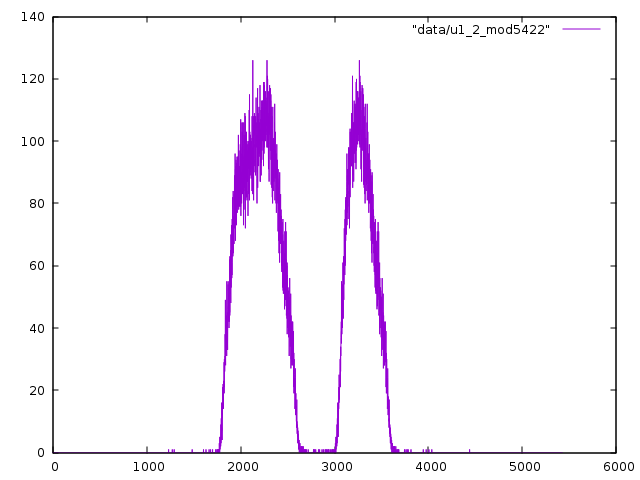
\includegraphics[scale=0.5]{../figs/u1_2_mod5422.png}

Supposing we look instead only at $a_n$'s for which 2, say is a summand.  Then we get this nice picture:

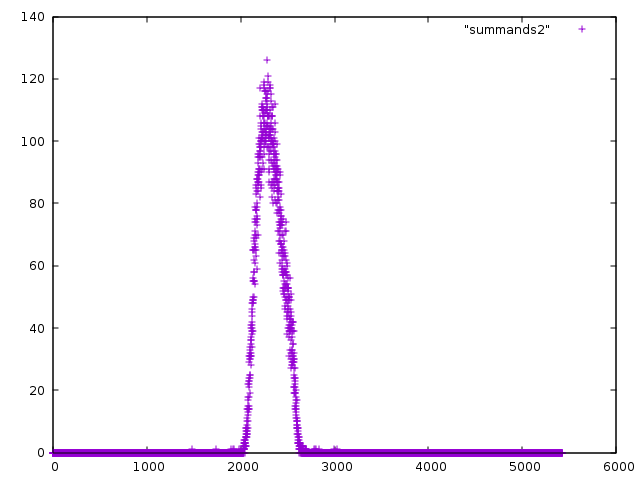
\includegraphics[scale=0.5]{../figs/summands2.png}

Likewise for 47:

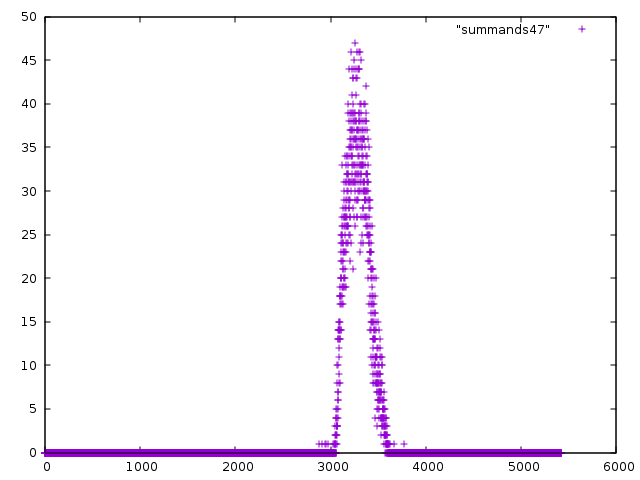
\includegraphics[scale=0.5]{../figs/summands47.png}

These are relatively clean-looking distributions, by comparison.  If
we plot these graphs for all of the top 25 most common summands all in
one picture, we notice that these seem to be the components of the two
observed peaks:

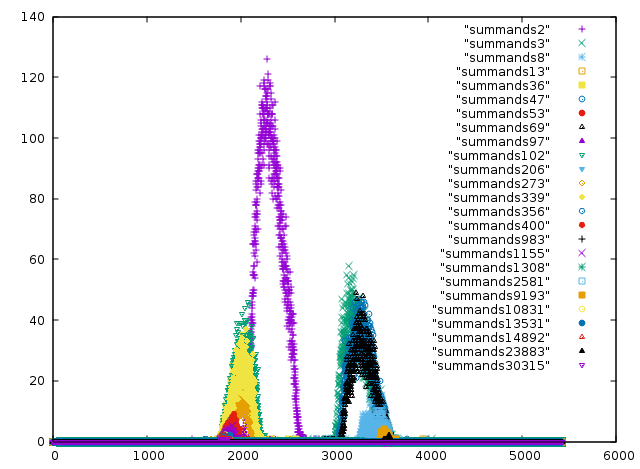
\includegraphics[scale=0.5]{../figs/summands_mod_5422.png}

Since each of these seems to be instances of the same distribution
with different parameters, we might be interested in computing the
parameters of each, starting with the means.  We do this with a crunchy bash script


% for x in `ls`; do y=$(echo $x|sed 's/summands//'); z=$(echo '('$(cat $x|sed 's/\([0-9]\)[ \t]\+\([0-9]\)/\1*\2/' | tr '\n' '+' | sed 's/+$//;s/[ \t]//g')')/'$(cat $x|awk '{x
  % +=$2} END {print x}')|bc -l);  echo -e "$y\t$(((y*2219)%5422))\t$z"; done|sort -n -k 2


Which outputs the summand $a_i$, the quantity $2219*a_i mod 5422$,
and the calculated mean of the distribution of $2219*a_n mod 5422$ for
which $a_i$ is a summand, we get:

\begin{tabular}{lll}
3	&1235	&3241.07886089813800657174\\
47	&1275	&3288.00715563506261180679\\
69	&1295	&3300.94546174403642482430\\
8	&1486	&3431.55542168674698795180\\
2581	&1607	&3485.87893462469733656174\\
983	&1633	&3503.28070175438596491228\\
206	&1666	&3518.47580645161290322580\\
1308	&1682	&3525.95679012345679012345\\
9193	&1703	&3541.35227272727272727272\\
13	&1737	&3551.59183673469387755102\\
23883	&1749	&3572.53333333333333333333\\
30315	&3653	&1818.70000000000000000000\\
13531	&3675	&1827.60000000000000000000\\
14892	&3680	&1833.36363636363636363636\\
10831	&3685	&1845.62962962962962962962\\
53	&3745	&1872.41395348837209302325\\
1155	&3761	&1883.37745098039215686274\\
356	&3774	&1878.85087719298245614035\\
97	&3785	&1891.29746835443037974683\\
400	&3814	&1912.78585086042065009560\\
273	&3945	&1984.79197207678883071553\\
36	&3976	&1995.70821114369501466275\\
339	&4005	&2013.33377814845704753961\\
102	&4036	&2027.29907648591049017286\\
2	&4438	&2319.24248003248950859618
\end{tabular}

Staring at this for a minute, we notice that if we subtract the second
column from the third, we seen to get roughly 2000 for the first 11
entries (those on the right end of the distribution).  Likewise, those
on the left end (rows 12-25) seem to have a similar pattern.

One possible source for this is that the distribution we're taking the
mean of in the first row, say, is of $2219*a_n mod 5422$ where 3 is a
summand of $a_n$ in the Ulam sequence.  Since 3 is a summand of $a_n$ in
the sequence, we might instead look at the other summand of $a_n$,
i.e. $a_n - 3$.  This would lead to us not plotting $2219*a_n mod 5422$,
but rather $2219*(a_n-3) mod 5422$.  We can compute these quickly with
another crunchy bash script [appendix A code 2]

And if we plot these, we get: 

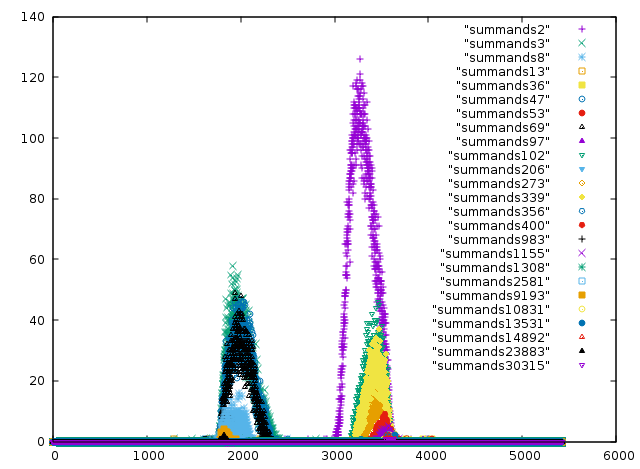
\includegraphics[scale=0.5]{../figs/shifted_summands_mod_5422.png}

That's more like it.  Running the same mean computation as above on this, we get:

\begin{tabular}{lll}
3    		&1235	&2006.0788\\
47   		&1275	&2013.0071\\
69   		&1295	&2005.9454\\
8    		&1486	&1945.5554\\
2581 		&1607	&1878.8789\\
983  		&1633	&1870.2807\\
206  		&1666	&1852.4758\\
1308 		&1682	&1843.9567\\
9193 		&1703	&1838.3522\\
13   		&1737	&1814.5918\\
23883		&1749	&1823.5333\\
30315		&3653	&3587.7000\\
13531		&3675	&3574.6000\\
14892		&3680	&3575.3636\\
10831		&3685	&3582.6296\\
53  		&3745	&3549.4139\\
1155 		&3761	&3544.3774\\
356  		&3774	&3526.8508\\
97   		&3785	&3528.2974\\
400  		&3814	&3520.7858\\
273  		&3945	&3461.7919\\
36   		&3976	&3441.7082\\
339  		&4005	&3430.3337\\
102  		&4036	&3413.2990\\
2    		&4438	&3303.2424\\
\end{tabular}

We note also that the picture kind of suggests a binomial distribution
because of the variance that appears to grow as the mean gets closer
to the middle.

Indulging this hypothesis for just a moment, the actual graph (say for
$a_i = 2$ specifically), is measuting "for each congruence class, how
many complements of 2 in the sequence are in that congruence class?"
The idea that this graph is a binomial distribution would be saying
that we can perform 5422 independent trials (say one for each
congruence class?)  with identical success probabilities (one possible
such test is pick randomly from the 100000 $a_n$s in that congruence
class and ask whether 2 is ever a complement of that $a_n$), and the
proportion of times 2 shows up as a complement of k is equal to the
proportion of times we get exactly k successes in our trials.


\subsection{Density}

The first step in our strategy is to establish positive density
results for sum-free and Ulam sequences.  In this paper, we will not
actually establish these, but give conjectures in this direction.
However, one may note that the only reason we know other Ulam
sequences such as $\ulam{2}{5}$ have positive density is that we know
they are regular.  So in trying to get a handle on the distribution
of, say, $\ulam{1}{2}$, it might seem backwards to start with an
assertion of positive density and then deduce regularity.

There are three things: 

\begin{enumerate}
\item First, it is already non-obvious that positive density in fact
  implies all the rest of what we want to know, and so even if this is
  all we can prove at the moment, it still seems worthwhile to record.
\item Second, beyond that, there is some reason for believing
  conjectures of this form.  Combined with a lot of experimental
  computations, one suggestive sort of argument takes the shape:
  ``There are many positive-density sets of the right sort
  (1-additive, sum-free, etc.), and the procedures for constructing
  the sum-free and Ulam sets that we are looking at are in some way
  `as greedy as possible', so what other sets could we get from those
  constructions if not some version of the positive-density ones we
  can construct?''  We will suggest some possible more precise
  versions of this in what follows.
\item Finally, while literal positive-density makes the arguments
  nicer, Many of the statements we wish to make later do have versions
  that make sense without it (mostly by changing ``large'' from
  meaning ``large relative to $N$'' to ``large relative to $|A_N|$''),
  as we shall discuss later.
\end{enumerate}

The first question is to attempt to compute the density of the various
sum-free sets and Ulam sequences that we are studying.  

\subsubsection{Computations}

The prescribed method for computing sum-free sets from a decision
sequence is already decently fast, provided we keep track of the data
appropriately.  Recall, the approach is to track three sets: $A$, the
actual sum-free set we are constructing, $D$, the set $A+A$ of things
that are ``disqualified'' from appearing in $A$, and $E$, the set of
things that are not disqualified by virtue of being sums but that,
according to the decision sequence, we are nevertheless to exclude.

We thus store $A$ as a list and $D$ as a hashset, (and need not keep
track of $E$).  So the algorithm is to, for each $x$ starting from 1
until we get bored:

\begin{enumerate}
\item Check if $x \in D$ (very fast, as $D$ is a hashset).  
\item If not, pop an item off the decision sequence.  
\item If 1, append $x$ in $A$ and add $x + A$ to $D$ ($|A|$ steps).
\end{enumerate}

So this algorithm to compute the first $N$ items will be roughly
$O(N \cdot |A_N|)$

A similar algorithm can be implemented for the Ulam sequence, in fact:
Now, we track the set $A$ as a list, the hashset $D$ of disqualified
items (i.e. $x$ for which $r^*_{A+A}(x) > 1$), the sorted list $C$ of
candidates (i.e. $x$ bigger than every element of $A$ with
$r^*_{A+A}(x) = 1$), and a hashset $C'$ that also contains the candidates.  Then the algorithm is to initialise the
following: 

\begin{enumerate}
\item $A = [a,b]$
\item $C = [a+b]$
\item $C' = \{a+b\}$
\end{enumerate}

And proceed thus: 

\begin{enumerate}
\item Delete any inital elements of $C$ that are smaller than the
  largest element of $A$.  As we go, delete these elements from $C'$
  also.
\item Let $x$ be the first element of $C$, and append $x$ to $A$.
\item For each $a \in A$: Compute $x + a$ and, if it is in $C'$,
  delete it from $C'$ (fast, since $C'$ is a hashset) and from $C$
  (where we can find it by bisection, since $C$ is sorted).
\end{enumerate}

There is a more advanced algorithm that leverages the apparent
regularity of such sequences as well, implemented in
\cite{knuth_algorithm}, which speed this basic algorithm up by, among
other things, noting that if we track which elements of $A$ are
outside the middle third mod $\lambda$ for a $\lambda$ where there are
few such elements, then when we're testing whether any new $x$ within
the middle third is actually a sum of smaller elements of $A$, we only
have to look at whether $x - a$ is in $A$ where $a$ is one of the
(hopefully few) elements of $A$ outside the middle third.  In fact,
one can be even more careful about it, which is done in
\cite{knuth_algorithm}.

In any case, the results of our computations give the following
estimates for the densities of these sets: 

{\color{red}[COMPUTATIONS]}

\subsubsection{Constructions}

We first start by noting that positive-density sum-free sets are
abundant, as a result of the abundance of sum-free sets
$A \subseteq \R/\Z$, coupled with the fact that if
$\pi_\lambda : \Z^+ \to \R/\Z$ by
$x \mapsto \frac{x}{\lambda} \mod{1}$, the inverse image
$\pi_\lambda\inv(A)$ is sum-free in the integers.  For example, the
set $A = \{1/2\}$ is sum-free in $\R/\Z$, and $\pi_2(A)$ is the odd
positive integers, which is sum-free.  Likewise, the $A_\lambda$ from
earlier (for any irrational $\lambda$), where recall $A_\lambda$ was
the set of integers that, when reduced (in $\R$) modulo $\lambda$,
land in the interval $(\frac{\lambda}{3}, \frac{2\lambda}{3})$, are
also of this form.  So this kind of example gives many sum-free sets,
both regular and irregular, that all have positive density.

One might wonder whether we can similarly generate examples of
Ulam-like sets of positive density.  It turns out that one can do this
using the basic idea behind the $A_\lambda$ construction, but being
more careful about it.  But first, we will make precise what we mean
by ``Ulam-like'': 

Recall an Ulam sequence is an increasing sequence of positive integers
that starts with some $a$ and $b$ and that continues by choosing
integers according to the requirements of 1-additivity (``every
element is uniquely a sum of previous elements'') and greediness
(``always choose the smallest such element available'').  In some
ways, it is the greediness that makes Ulam sequences hard to analyse.
If we drop this condition, then we get a general class of sequences to
which belong the Ulam sequences, but also many others:

\begin{definition}\label{def:1additive}
  For $S \subseteq \Z^+$ a finite set (say of size $k$), a
  \textbf{1-additive sequence with base $S$} is an infinite sequence
  of positive integers $a_i$ such that $a_1 < \ldots < a_k$ are the
  elements of $S$, and, for $n > k$, $a_n$ is greater than $a_{n-1}$
  and has a unique pair of integers $i, j$ with $0 < i < j < n$ such
  that $a_n = a_i + a_j$.

  We may talk of simply a \textbf{1-additive sequence}, by which we
  will mean a sequence of integers that is a 1-additive sequence with
  base $S$ for some $S$.
\end{definition}

\begin{example}
  \begin{enumerate}
  \item Any Ulam sequence $U(a,b)$ is 1-additive with base $a, b$.  
  \item The Fibonacci numbers $1, 2, 3, 5, 8, \ldots$ are a 1-additive
    sequence with base $1, 2$.  
  \item The set $\{2, 3, 5, 7, 9, \ldots\} = 2, 2+3\Z^+$ is 1-additive
    with base $2, 3$.  
  \item More generally, for any $a < b$, the set $a, b, b+a, b+2a,
    \ldots$ is 1-additive provided $b \neq 0 \mod{a}$.  
  \end{enumerate}
\end{example}

The last example gives plenty of examples of regular 1-additive
sequences.  But we might wonder what the analogue of $A_\lambda$ (for
irrational $\lambda$ would be for 1-additive sets.  Indeed, these were
our first examples of irregular sum-free sets of positive density, so
we might first ask whether there even is such a thing for 1-additive
sets.  It turns out that there is: 

\begin{proposition}
  There exists an irregular 1-additive set of positive density.
\end{proposition}

\begin{proof}[Idea of proof]
  The basic idea will be the following ``ping-pong mod $\lambda$''
  construction: Take an irrational $\lambda$.  Take $a$ (the ``left
  bat'') just above $0$ mod $\lambda$, and $b$ (the ``right bat'')
  just below 0 mod $\lambda$, and a $c$ (the ``ball'') just above
  $\lambda/3$ mod $\lambda$.  The game will be to keep the ball in the
  set $T = (\frac{\lambda}{3}, \frac{2\lambda}{3})$ (the ``table'')
  mod $\lambda$ by adding $a$ to it until it reaches the right side,
  then adding $b$ to it until it reaches the left side, and repeating
  indefinitely.

  Supposing we are a little careful about our choices of $a, b, c$,
  and $\lambda$, we should be able to show that this construction
  satisfies the required properties.
\end{proof}

\begin{proof}
  More precisely: start with an irrational $\lambda$, an $a$ with
  $a \mod{\lambda}$ lying in $(0, \frac{\lambda}{12})$, and a $b > a$
  with $b \mod{\lambda}$ in $(\frac{11\lambda}{12},\lambda)$, and a
  $c$ with $c \mod{\lambda}$ in $(\frac\lambda 3, \frac\lambda 2)$,
  and say further that $a \nmid b$ (for reasons that will become
  apparent later).

  Then we will define a sequence of sets $A_n$ which will comprise the
  sequence $A$, as follows: Let $c_1 = c$.  For $n \geq 1$, let
  $A_n = \{c_n + ka : k \in \Z^+, c+ka\mod{\lambda} \in T\}$, and let
  $c_{n+1}$ be the largest element of this set (allowing the
  definition of $A_{n+1}$ to make sense).  

  Then let $S = \{a, b, c\}$ and $A = S \cup \bigcup_{i=1}^\infty
  A_i$.  

  Now let us check the definition: Our base set is $S$.  Every element
  $a_i$ has $a_i < a_{i-1} + a + b$, so the set is has positive
  density.  This set is not dense mod $\lambda$, but any regular set
  would have to be (since $\lambda$ is irrational), so $A$ cannot be
  regular.  It remains to check 1-additivity.  

  By construction, every element $a_n > c$ is either $a_{n-1} + a$ or
  $a_{n-1}+b$, so every element not in $S$ is a sum of smaller
  elements in at least one way.  Now suppose $a_n$ is a sum of smaller
  elements in another way also.  Then because $a_n$ is in the middle
  third, it cannot be a sum of two other elements in the middle third.
  Thus the only for $a_n$ to be a sum of other elements of $A$ in two
  different ways is if $a_n - a$ and $a_n - b$ are both in $A$.  

  But now, say $a_n = c + ax + by$, for some $x \geq 0, y \geq 0$.
  We know either $a_n - a \in A$ or $a_n - b \in A$.  If $a_n - b \in
  A$, Then by definition, the next element of $A$ will be $a_n$, and
  $a_n - b < a_n - a < a_n$, so $a_n - a$ cannot be in $A$.  

  If instead $a_n - a \in A$, then say the place where we started
  adding $a$s (before $a_n$) was $r$ steps back ($r \geq 1$ since
  $a_n - a \in A$), i.e. at $c + a(x-r) + by$.  Then the element
  before this in $A$ would be $c + a(x-r) + b(y-1) < a_n - b$.  Thus
  for $a_n - b$ to be in $A$, it would have to be an element after
  $c + a(x-r) + b(y-1)$, i.e. an element of the form
  $c + a(x-s) + by$.  But $c + a(x-s) + by = c + ax + by - b$ implies
  $as = b$, which contradicts $a \nmid b$, which was our condition on
  $a$ and $b$.  

  Thus $a_n - a$ and $a_n - b$ can never both be in $A$, making $A$
  also 1-additive.
\end{proof}

We note, however, that this construction gives us a 1-additive set
with a base of size 3, whereas the Ulam numbers are a 1-additive set
with a base of size 2.  So we might wonder whether there is a similar
(if more complicated) construction of this sort.

The following construction, we believe should work: 

\begin{conjecture}
  There is an irregular, positive density 1-additive set with a base
  of size 2.
\end{conjecture}

\begin{proof}[Idea]
  We will play the same game of ping-pong, but now we are only allowed
  to use two elements.  We will again start with an irrational
  $\lambda$ and $a \in \Z^+$ the ``left bat'' in the range
  $(\frac{\lambda}{6}, \frac{\lambda}{3})$ mod $\lambda$.  But now we
  will start with $c$ being the ``ball'' inside the ``table''
  $T = (\frac{\lambda}{3}, \frac{2\lambda}{3})$.

  Then we will add $a$ to $c$ until it comes out on the right side as
  some $b \in (\frac{2\lambda}{3}, \frac{5\lambda}{6})$, and that will
  be our ``right bat''.  Then we will do roughly the same thing as
  before, except now $a$ and $b$ have larger magnitude mod $\lambda$,
  so they may occasionally hit the ball off the table slightly.  This
  will give us further bats with which to hit the ball--usually bats
  with even greater magnitude mod $\lambda$.  The idea, then, will be
  to always hit the ball with the largest available bat that doesn't
  send it off the table (when possible), so that there is the most
  flexibility for the other side to ensure they are also able to hit
  the ball back onto the table.  
\end{proof}

\subsubsection{Conjectures}

Recall that sum-free sets of positive integers correspond bijectively
with binary ``decision'' sequences.  We know also that there are many
sum-free sets of positive density.  Further, we can easily see that if
the 1s have zero density in the decision sequence, then the resulting
sum-free set has zero density.  So all the positive-density sum-free
sets must have decision sequences with positive density.  

\begin{question}
  For any decision sequence $S$ with a positive density of 1s, the
  corresponding sum-free set $A = \theta(S)$ has positive upper density.
\end{question}

\begin{conjecture}
  For any decision sequence $S$ that is eventually periodic and for
  which the repeating pattern has at least one 1, then the
  corresponding sum-free set $A = \theta(S)$ has positive upper
  density.
\end{conjecture}

As we have said, it appears that the Ulam sequence has positive
(upper) density around $0.07$.  This, together with the ultimate
greediness of the Ulam sequence suggests for us the conjecture:

\begin{conjecture}
  The Ulam sequence $\ulam{1}{2}$ has positive upper density.
\end{conjecture}

\section{Future Directions}

\subsection{Reducing 1-additive sets to sum-free sets}

\subsubsection{Via triangle removal}

\subsection{Technology}

\subsubsection{Arithmetic regularity}

\subsubsection{Ultralimits}

\subsection{Variants of the Ulam problem}
\subsubsection{Larger seed sets}
\subsubsection{Sums of more than two previous elements}

Circle method gets better with more variables.  For this reason, we
might find it convenient to 

\subsubsection{Probabilistic versions}


% \section{Appendix A: Code}

% Code 1: 

% \begin{lstlisting}[language=Python]% {../lll.py}
% from sage.libs.fplll.fplll import FP_LLL
% b2=2.57144749848
% b=N(2*pi/2.57144749848)

% def find_mp(x,deg=50,n=10^10):
%     M = []
%     for i in range(deg+1):
%         M.append([1 if v == i else 0 for v in range(deg+1)]+[int(n*(x^i)+.5)])
%     M = matrix(M)
%     F=FP_LLL(M)
%     F.LLL()
%     l=F._sage_()[0][:-1]

%     R = ZZ["X"]
%     X=R.gen()
%     fx = 0
%     for i in range(len(l)):
%         fx += X^i * l[i]
%     ans = N(fx(x),50)
%     return(fx, ans, fx.factor())

% ms = [find_mp(b,i) for i in range(2,10)]
% ms.sort(key=lambda x:abs(x[1]))
% for x in ms:
%     print(x)

% print("")
% ms = [find_mp(b2,i) for i in range(2,10)]
% ms.sort(key=lambda x:abs(x[1]))
% for x in ms:
%     print(x)
% \end{lstlisting}

% Code 2: 

% \begin{lstlisting}[language=Bash]
% cat data/indices_of_summands | cut -d " " -f 4 | sort -n|uniq -c|sort -n > data/n_minus_js
% cat data/indices_of_summands | cut -d " " -f 3,4 | sort -n|uniq -c|sort -n > data/i_nmj
% \end{lstlisting}

\begin{thebibliography}{9}
\bibitem{ulam_steinerberger} 
Stefan Steinerberger\\
Hidden regularity

\bibitem{knuth_algorithm} 
Knuth\\
Algorithm for computing Ulam numbers
 
\bibitem{patterns_finch} 
Finch\\
Patterns in 1-additive sequences
 
\bibitem{regularity_criterion_finch} 
Finch
 
\bibitem{regularity_schmerl} 
Schmerl, Speigel
 
\bibitem{capset_ellenberg} 
Ellenberg, Gijswijt

\bibitem{progressions_croot} 
Croot, Lev, Pach

\bibitem{sumfree_cameron} 
Cameron

\bibitem{aperiodic_sumfree_erdos} 
Erdos65

\bibitem{sumfree_regularity_luczak} 
Luczak

\bibitem{avoid_zero_gibbs} 
Gibbs

\bibitem{difference_density_calkin} 
Calkin, Finch, Flowers\\
Difference Density and Aperiodic Sum-Free Sets 

\bibitem{additive_combinatorics_tao} 
Tao, Vu\\
Additive Combinatorics

\bibitem{no_large_sumfree_subset_eberhard}
  https://arxiv.org/pdf/1301.4579v2.pdf Eberhard, Green, and Manners

\bibitem{lyall_roth}
  Niel Lyall: Roth's theorem 

\bibitem{higher_fourier_analysis_tao}
  Tao, Higher Fourier Analysis

\bibitem{computations}
  https://github.com/daniel373592559/wip-ulam/experiments.py

\end{thebibliography}

}

\end{document}